\documentclass[phd,bottom,nosig]{usbthesis}

\usepackage{mathtools}
\usepackage{amssymb}
\usepackage{amsfonts}
\usepackage{amsthm}
\usepackage{bm}


\usepackage{graphicx}
\usepackage{float}
%\usepackage{tikz}
\usepackage{array}
\usepackage{tabularx}
\usepackage{multirow}
\usepackage{hhline}

% 算法环境
\usepackage{algorithm}
\usepackage{algpseudocode}

% 文本与布局
\usepackage{setspace}
\usepackage{afterpage}
\usepackage{footmisc}
\usepackage{xspace}
\usepackage{enumitem}
\usepackage{comment}

% 引文
\usepackage[numbers,sort&compress]{natbib}

% 颜色与 caption
\usepackage{xcolor}
\usepackage{caption}
\usepackage{subcaption}

% 其他
\usepackage{pdfpages}
%\usepackage{silence}
%\WarningFilter{revtex4-1}{Repair the float}

% 超链接放最后
\usepackage{hyperref}
\hypersetup{
    colorlinks=true,
    linkcolor=blue,
    filecolor=magenta,
    urlcolor=cyan,
    citecolor=blue
}

\renewcommand{\thesubsection}{\thesection.\arabic{subsection}}
\makeatletter
\renewcommand{\p@subsection}{}
\makeatother

\newtheorem{definition}{Definition}
\newtheorem{lemma}{Lemma}
\newtheorem{proposition}{Proposition}
\newtheorem{theorem}{Theorem}

%\usepackage[nottoc]{tocbibind}
\input{mathdefs}
\input{callcommands}
\hyphenation{put words here which LaTeX does not hy-phen-ate pro-per-ly}

\author{Hongji Gao}%
\title{Asymptotic-Behavior–Driven Algorithm Design and Discrimination: From Scalable Computation to Convergence Metrics}%

\month{December}
\year{2025}%
\program{Applied Mathematics and Statistics}%
\director{Xiangmin Jiao}{Professor, Department of Applied Mathematics and Statistics}%
%\chairman{Name of Chairman}{Professor, Department of Physics and Astronomy}%
\chairman{Robert~Harrison}{Professor,  Institute for Advanced Computational Scinece}%
%\fstmember{Name of Member}{Professor, Department of Physics and Astronomy}%
\fstmember{Benjamin~Levine}{Professor, Department of Chemistry}%
%\outmember{Name of Outside Member}{Position}{Institution}%
\outmember{Name of Outside Member}{Position}{Institution}%
\dean{Eric Wertheimer}%

\begin{document}

\singlespacing %
\pagenumbering{roman} %
\maketitle %
\makeapproval %

\begin{abstract}
Post-Hartree--Fock methods are often limited by the storage and repeated use of large tensors: wavefunction coefficient objects in configuration-interaction (CI) calculations and the electron--repulsion integral (ERI) tensor in perturbative correlation. Most entries of these matrices are small in absolute value, but treating the matrices as strictly sparse by aggressive elementwise truncation can be too crude. Hierarchical compression offers an effective middle ground, combining blockwise sparsity with locally controlled low-rank structure to reduce memory and accelerate dominant contractions while retaining systematic accuracy control.

We develop two hierarchical methods tailored to distinct bottlenecks. For complete active space and full configuration interaction, we introduce corner hierarchically approximated configuration interaction (CHACI), which compresses the CI vector using corner hierarchical partition, norm-based sorting, and blockwise rank selection to maximize information density. By application to dodecacene, a strongly correlated molecule, we demonstrate that corner hierarchical matrix compression provides superior compression compared to a truncated global singular value decomposition. For M\o ller--Plesset perturbative methods, we present a hierarchical SOS-MP2 algorithm that applies $\mathcal{H}^{2}$ compression to the ERI tensor within an atomic-orbital Laplace framework, leveraging sparsity in energy-weighted density matrices. The resulting method achieves $\mathcal{O}(N^{2}\log N)$ time and space complexity for the Coulomb-like SOS-MP2 term and exhibits even better scaling on linear alkanes and three-dimensional water clusters with $N$ as the number of basis sets.

\end{abstract}
\tableofcontents %
\listoffigures %
%
%\listoftables %
%
\begin{acknowledgements}
    First and foremost, I would like to express my deepest gratitude to my advisor, Professor Xiangmin Jiao.
His exceptionally clear vision of the field and patient guidance have been invaluable throughout my Ph.D.\ journey. Under his mentorship, I have significantly strengthened my mathematical foundation and greatly improved my coding skills. His genuine passion for academic research consistently inspired me and helped shape both my research direction and my growth as an independent scholar.

I am also profoundly grateful to my co-advisor, Professor Benjamin Levine, for his insightful guidance in chemistry and for the tremendous effort he devoted to paper writing and responses. I would like to thank Professor Harrison and the Institute for Advanced Computational Science (IACS) for providing funding and, more importantly, for offering opportunities that broadened my academic horizons and enabled meaningful scholarly exchanges. I sincerely thank my thesis chair, Professor Roman Samulyak, and my committee member, Professor Marivi Fernandez-Serra, for their careful reading of my dissertation and for the time, energy, and thoughtful suggestions they contributed to improving this work.

I would like to thank all the present and past members of my research group, including Yipeng Li, Qiao Chen, Xuebin Wang, Jacob Jones, and Chao Zhang, for the many helpful discussions, feedback, and support during group meetings.
I also gratefully acknowledge my collaborators on my Ph.D. projects, including Kenneth Berard and Ying You.
Without their contributions, it would have been much more difficult to complete this work so efficiently.

Finally, I would like to thank my parents for their unconditional love and support. I am especially grateful to my girlfriend, Tianyi Chen, for her understanding, encouragement, and companionship. I also thank my friends in Stony Brook, including Fengchun, Zelong, Yuqi, Zhixing, Chengpeng, Yushen, Wenhan, Sijia, Josh, Zhengxiang, Cheng and many others, for making my life during this time meaningful and joyful.
\end{acknowledgements}
\pagestyle{thesis}
\newpage
\pagenumbering{arabic}
\chapter{Introduction}

Post-Hartree--Fock (post-HF) electronic structure methods are essential for reaching quantitative accuracy in molecular systems' energy and properties, yet their practical reach is often limited by the cost of manipulating large operators and high-dimensional tensors. In modern implementations, this limitation is not solely a matter of floating-point operations: memory footprint, data movement, and unfavorable scaling in the dominant contractions frequently determine feasibility. A common observation across correlation methods is that the key objects are rarely ``generic dense.'' They typically exhibit \emph{structured sparsity} and \emph{structured compressibility} induced by physical locality, screening, and the organization of electronic degrees of freedom. The central aim of this dissertation is to turn these latent regularities into concrete algorithmic gains by designing hierarchical compression techniques that reduce the leading-order time and memory costs while retaining controlled accuracy.

Hierarchical matrices provide a particularly suitable framework for this goal because they interpolate between two extremes that are both unsatisfactory in many chemical settings. Pure sparse-matrix treatments assume that a large fraction of entries are exactly zero (or can be set to zero without consequence), and they therefore operate only on the remaining nonzeros. This is highly effective when the underlying operator truly induces sparsity. However, for many operators and tensors in electronic structure, aggressively zeroing small entries is too blunt: entries may be individually small but collectively important, and truncating them entrywise can destroy delicate cancellations or bias energy differences. At the other extreme, dense representations avoid approximation but quickly become memory- and bandwidth-bound as system size grows. Hierarchical matrices occupy the middle ground and should be viewed as a \emph{structure-aware sparse representation}: the matrix is sparse at the level of blocks (most blocks are not stored densely), but rather than discarding entire regions or entries, one replaces selected blocks by low-rank surrogates whose error is locally controlled. In other words, hierarchical matrices treat many chemically relevant objects as ``sparse, but not sparse enough to be treated as strictly sparse'' and exploit additional distributional regularities---such as concentration near a diagonal band, within a localized region, or in a small principal corner---to compress the remainder in a principled way.

Concretely, hierarchical matrix formats recursively partition the index sets into a multilevel cluster tree and thereby induce a block partition of the matrix. Near-field blocks (or blocks in regions of high information density) are kept explicitly, often still sparse or moderately dense depending on the application. Far-field blocks (or blocks in regions where information is diffuse) are approximated by low-rank factorizations. Classical H-matrices already yield substantial reductions in storage and matrix--vector multiplication by exploiting this blockwise low rank. The H$^2$ variant strengthens the representation further by introducing \emph{nested bases}: low-dimensional subspaces are shared across multiple blocks and reused across hierarchy levels. This nested structure is crucial when the same operator must be applied repeatedly inside iterative solvers or correlation pipelines, because it amortizes the cost of basis construction and reduces both memory and application complexity under mild rank-growth assumptions. Importantly, hierarchical matrices do not impose a single global rank or a single global notion of ``importance.'' They provide a language to encode heterogeneity: different parts of the matrix can be represented at different resolutions and with different ranks, guided by local error tolerances and local structural cues.

These properties have made hierarchical techniques broadly relevant in computational chemistry, where central objects naturally exhibit locality and screening. A prominent example is the four-index electron--repulsion integral (ERI) tensor, which can be reshaped into an $N^2\times N^2$ matrix (with $N$ the number of one-electron basis functions) indexed by basis-function pairs. In localized orbital or atomic-orbital bases, ERIs display strong near-field structure: interactions among nearby orbital pairs are comparatively strong and must be represented accurately, while interactions between well-separated groups are often compressible and admit low-rank descriptions. Hierarchical representations exploit exactly this separation, enabling reduced-memory integral storage and accelerating the construction and application of Coulomb- and Fock-like intermediates. More generally, hierarchical methods exemplify a guiding principle that is central to this dissertation: global algorithmic improvements follow from local, quantifiable structure, provided that the data layout, the approximation format, and the computational kernels are designed together so that the structure is exposed and reused across scales.

The focus of this dissertation is on hierarchical compression techniques for two representative post-HF bottlenecks that embody two \emph{different} kinds of structure. The first bottleneck arises in configuration-interaction (CI) approaches for strongly correlated systems, where the size of the coefficient tensor (or its matricizations) becomes memory-limiting as active spaces grow. The second bottleneck arises in perturbative correlation methods such as second-order M{\o}ller--Plesset theory (MP2), where the ERIs dominate both storage and contraction cost. While both objects can be viewed through the lens of large matrices (via unfoldings or reshaping), their compressibility is governed by different organizing principles: CI coefficients are primarily structured by excitation patterns and wavefunction weight distribution, whereas ERIs are primarily structured by spatial locality. A central message that emerges from the two works integrated here is that \emph{the best hierarchical format is problem-dependent}: one should not expect a single partitioning strategy (e.g., diagonal-centric admissibility) to be optimal for all post-HF objects.

To motivate the wavefunction side, recall that truncated CI methods represent the correlated state as a linear combination of determinants. In practice, the coefficient object is not merely a vector; it is frequently manipulated through structured decompositions, and a particularly informative organization is obtained by grouping determinants into $\alpha$- and $\beta$-spin strings. This yields a coefficient matrix $C$ whose rows index $\alpha$-strings and columns index $\beta$-strings. Empirically, such matrices often exhibit a striking nonuniformity: a relatively small subset of configurations carries most of the wavefunction weight, and under suitable orderings this nonuniformity manifests as a \emph{corner-dominant} pattern in $C$, where the most significant entries concentrate near a principal corner and decay away from it. This pattern is neither classical sparsity (exact zeros) nor the type of diagonal dominance that standard hierarchical formats implicitly privilege. It is instead an anisotropic concentration of information, suggesting that the hierarchy itself should be aligned with the corner where the signal resides.

The first major contribution of the dissertation therefore develops a \emph{corner-hierarchical} representation and the associated compression algorithm CHACI (CH-based approximated configuration interaction). The key design decision is to replace a ``uniform'' or ``diagonal-first'' partition by a hierarchy that recursively refines the corner region where information density is highest. Within this structure, CHACI performs blockwise compression and chooses between dense storage and truncated SVD (TSVD) representations on a per-block basis, guided by the principle that a block should be stored in the form that yields the most retained wavefunction information per unit memory at the target tolerance. A crucial practical ingredient is a data-reordering step: rows and columns are sorted by their $\ell_2$ norms so that large-magnitude rows and columns move toward the privileged corner, intensifying the corner concentration that the hierarchy is designed to exploit. Another key ingredient is \emph{rank adaptivity}: rather than imposing a single global rank (which wastes degrees of freedom in unimportant regions and starves important regions), CHACI selects ranks locally according to an information-density criterion derived from singular values and storage costs, and it allows blocks to remain dense when low-rank representation is not beneficial. Because CI coefficients must also satisfy global constraints (e.g., normalization) and because truncation error can redistribute weight across blocks, CHACI further incorporates blockwise normalization procedures that stabilize the compressed representation and mitigate artificial population transfer that would occur under a single global renormalization. The net effect is a compression strategy that is tailored to the observed geometry of information in CI tensors: it aims to capture more signal per stored parameter than global low-rank factorizations of the same unfolding and to do so in a way that remains compatible with downstream CI manipulations.

Where CHACI is driven by anisotropic coefficient concentration, the second contribution is driven by geometric far-field compressibility of the ERI operator, with the ultimate goal of accelerating MP2 correlation. MP2 provides a widely used description of dynamic correlation as a second-order perturbative correction to the Hartree--Fock reference. Although MP2 is cheaper than higher-level coupled-cluster methods, canonical formulations still involve expensive contractions and are heavily constrained by ERI storage and transformation. The approach developed in this dissertation targets the spin-opposite-scaled variant (SOS-MP2), which focuses on opposite-spin (Coulomb-like) contributions and is particularly amenable to atomic-orbital formulations. The central idea is to represent the reshaped ERI tensor as an H$^2$ matrix, leveraging a near-/far-field split: near-field blocks (including diagonal and nearby interactions) are handled explicitly or with mild compression, while far-field blocks are represented in low rank with nested bases to maximize reuse across the hierarchy. This hierarchical ERI representation is then coupled to an AO Laplace-transform formulation of SOS-MP2, in which the correlation energy is expressed as a weighted sum over quadrature points. At each quadrature node, the computation reduces to applying the ERI operator to structured auxiliary quantities constructed from energy-weighted density-like matrices. These auxiliary matrices exhibit additional sparsity in large finite systems due to spatial decay; by truncating small elements below a user tolerance and storing them in sparse formats (e.g., CSR), the algorithm restricts work to the chemically relevant entries while still accounting for the long-range contributions through the compressed ERI operator rather than discarding them. A further organizational feature is a short-/long-range decomposition of the ERI operator within the hierarchical format, enabling separate index transformations for near-field and far-field contributions and an efficient recombination in the trace expressions that define the SOS-MP2 energy. In this way, the method replaces dense tensor contractions by hierarchical operator applications and small dense kernels, with accuracy controlled by local block tolerances and rank adaptivity in the H$^2$ representation together with quadrature parameters in the Laplace factorization. The overarching outcome is a correlation pipeline whose dominant stages are governed by hierarchy traversal and nested-basis arithmetic rather than by unstructured dense algebra.

Taken together, the two methods illustrate a coherent design philosophy for hierarchical compression in post-HF electronic structure: (i) identify the dominant structural regularity of the target object, (ii) select or develop a hierarchical format whose partitioning strategy aligns with that regularity, and (iii) embed local error control into the representation and kernels so that accuracy is achieved through interpretable tolerances rather than through ad hoc global heuristics. CHACI emphasizes that, for wavefunction objects, the correct notion of ``near field'' may be an information-theoretic region (a corner of high coefficient density) rather than a geometric one, and that reordering and blockwise rank selection are essential for turning empirical concentration into reliable memory savings. The H$^2$-AO-SOS-MP2 pipeline emphasizes that, for operator objects such as ERIs, geometric locality and far-field low rank can be exploited most effectively when nested bases are reused across levels and when the surrounding correlation algorithm is reformulated so that its dominant operations become repeated applications of the compressed operator.

The dissertation is organized to develop these contributions from a shared foundation and to connect their design choices to reproducible computational benefits. We begin with preliminaries that establish the hierarchical-matrix background needed throughout, including hierarchical partitioning, admissibility concepts, blockwise low-rank approximation, nested bases in H$^2$ formats, and the primitives for compression, traversal, and error control. We also summarize the electronic-structure context required to situate the two compression targets, including the organization of CI coefficient tensors via $\alpha$--$\beta$ string decompositions and the reshaping of ERIs into pair-space operators. Building on these preliminaries, we first present the CHACI method for compressing FCI (and related active-space CI) coefficient tensors: the corner-hierarchical format, the sorting and normalization procedures, the adaptive rank-selection strategy based on information density, and numerical studies that demonstrate favorable storage--accuracy trade-offs as active spaces grow. We then present the H$^2$-AO-SOS-MP2 method for ERI compression and MP2 acceleration: the H$^2$ data structures and near-/far-field split, the AO Laplace formulation, the sparse treatment of auxiliary matrices, the hierarchical index transformations, and the resulting complexity and accuracy behavior. Finally, we conclude by synthesizing the two contributions under a unified viewpoint: hierarchical compression is most effective when the representation is matched to the geometry of information in the object being approximated---corner concentration for CI coefficients and far-field low rank for ERIs---and when local error control is integrated into the computational pipeline so that chemical accuracy can be reached with predictable resource usage.
\chapter{Preliminaries and Related Work}
\label{sec:prelim}
\subsection{Hierarchical matrices}
\label{subsec:h-matrix}

Hierarchical matrices ($\mathcal{H}$-matrices) are data-sparse representations
for large, structured matrices arising in applications such as elliptic partial
differential equations, boundary integral equations, and kernel methods
\cite{HackbuschBorm2002,Bebendorf2008,Hackbusch2015}. The main idea is to
exploit the fact that matrix blocks corresponding to well-separated index
clusters are often numerically low rank, while blocks corresponding to
near-field interactions are not.

More precisely, one first organizes the index set
$\mathcal{I} = \{1,\dots,N\}$ into a cluster tree based on geometric or
algebraic information, and then constructs a block cluster tree that partitions
the $N\times N$ matrix into blocks. An admissibility condition---typically
expressing that the underlying index clusters are well separated---is used to
classify blocks as \emph{far-field} or \emph{near-field}. Near-field blocks are
stored explicitly as dense matrices, while far-field blocks are compressed by
low-rank approximations, often obtained by SVD, RRQR, or SRRQR.

Under mild assumptions on the underlying problem and the admissibility
condition, $\mathcal{H}$-matrices achieve almost linear storage and arithmetic
complexity. For example, for a second-order elliptic operator in three
dimensions, one can typically store the corresponding stiffness matrix in
$\mathcal{O}(N \log N)$ memory and apply it to a vector in
$\mathcal{O}(N \log^2 N)$ time, where $N$ is the number of degrees of freedom
\cite{Hackbusch2015}. In the language of Section~\ref{subsec:asymptotic}, this
represents a substantial improvement over the $\Theta(N^2)$ storage and
$\Theta(N^2)$ matrix-vector multiplication cost of a dense matrix.

The hierarchical organization is particularly flexible: blocks can be further
subdivided, admissibility can be adapted to the problem at hand, and different
low-rank approximation techniques can be used in different parts of the
matrix. This flexibility makes $\mathcal{H}$-matrices a natural tool for
compressing large matrices and tensors in many-body problems.

\subsection{$\mathcal{H}^2$-matrices}
\label{subsec:h2-matrix}

While $\mathcal{H}$-matrices already reduce storage and computation costs
significantly, they store separate low-rank bases for different far-field
blocks, which leads to redundancy. $\mathcal{H}^2$-matrices refine this idea by
introducing \emph{nested} cluster bases that are shared across blocks
\cite{BormGrasedyckHackbusch2003,Hackbusch2015}. In an $\mathcal{H}^2$-matrix,
each cluster in the index tree is associated with a basis that spans the
relevant far-field interactions, and bases at coarse levels are represented in
terms of bases at finer levels via small transfer matrices.

This nested structure eliminates much of the redundancy present in standard
$\mathcal{H}$-matrices. Under suitable assumptions on the kernel or operator,
$\mathcal{H}^2$-matrices can achieve linear or nearly linear complexity:
\begin{equation}
  \mathcal{O}(N) \quad\text{for storage}, \qquad
  \mathcal{O}(N) \quad\text{for matrix-vector multiplication},
\end{equation}
again up to logarithmic factors and assuming bounded ranks. From the asymptotic
viewpoint, this represents an improvement from $\mathcal{O}(N \log N)$ or
$\mathcal{O}(N \log^2 N)$ to (essentially) $\mathcal{O}(N)$, while maintaining
a prescribed accuracy in the relevant matrix norm.

$\mathcal{H}^2$-matrices are particularly effective for discretizations of
translation-invariant or asymptotically smooth kernels, such as Green's
functions of elliptic operators and Coulomb-like interactions. In later
chapters we will make use of hierarchical and $\mathcal{H}^2$-matrix ideas to
compress large matrices and tensors arising in electronic-structure theory,
and we will analyze their storage, computational complexity, and approximation
errors using the asymptotic framework introduced in
Section~\ref{sec:prelim-convergence}.

\section{Quantum Chemistry Background}
\label{sec:prelim-chem}

We now review the quantum chemistry background relevant to this work, focusing
on the tensor structures and electronic-structure methods that will be used in
later sections. We first introduce the full configuration interaction (FCI)
tensor and the electron repulsion integral (ERI) tensor, and then briefly
review the Hartree--Fock (HF) method and second-order M{\o}ller--Plesset
perturbation theory (MP2). Throughout, we emphasize the asymptotic behavior of
the computational cost in terms of the number of basis functions and electrons.

\subsection{Full configuration interaction tensor}
\label{subsec:fci-tensor}

Consider an $N$-electron system in a finite one-particle basis of $M$
spin-orbitals $\{\chi_p\}_{p=1}^M$. Within this basis, the electronic
wave function can be expanded in a basis of Slater determinants
$\{\Phi_I\}$ constructed by occupying $N$ spin-orbitals out of $M$:
\begin{equation}
  \Psi
  = \sum_{I} C_I \Phi_I,
  \qquad
  \Phi_I = \frac{1}{\sqrt{N!}}
  \det\bigl[\chi_{i_1}(1)\,\chi_{i_2}(2)\,\dots\,\chi_{i_N}(N)\bigr],
\end{equation}
where $I = (i_1,\dots,i_N)$ indexes the occupied spin-orbitals in determinant
$\Phi_I$ and $C_I$ are configuration interaction (CI) coefficients. In full
configuration interaction (FCI), the sum runs over all determinants consistent
with the specified number of electrons and spin symmetry, leading to a formally
exact solution of the nonrelativistic electronic Schr\"odinger equation within
the chosen basis \cite{SzaboOstlund1989,HelgakerJorgensenOlsen2000}.

The dimension of the determinant basis is
\begin{equation}
  N_\mathrm{det}
  = \binom{M}{N_\alpha} \binom{M}{N_\beta},
\end{equation}
where $N_\alpha$ and $N_\beta$ are the numbers of $\alpha$- and $\beta$-spin
electrons, respectively. As $M$ grows, $N_\mathrm{det}$ increases
combinatorially, which leads to an exponential scaling of the FCI cost with
respect to system size. In the asymptotic language of
Section~\ref{subsec:asymptotic}, the storage required for the CI coefficients
is $\Theta(N_\mathrm{det})$, which behaves roughly like
$\exp(\mathcal{O}(M))$ for fixed electron fraction.

It is often convenient to view the collection of CI coefficients as a tensor,
the \emph{FCI tensor}. For example, in an occupation-number representation the
FCI tensor has one index per spin-orbital,
\begin{equation}
  C_{n_1 n_2 \dots n_M},
  \qquad n_p \in \{0,1\},
\end{equation}
subject to the constraint $\sum_p n_p = N$. Alternatively, one can group
spin-orbitals into $\alpha$- and $\beta$-strings and fold the CI vector into a
matrix with indices $(I_\alpha, I_\beta)$, where each index labels an
occupation pattern of $\alpha$- or $\beta$-spin orbitals. Regardless of the
specific indexing, the resulting FCI tensor is extremely high-dimensional and
dense, and serves as a prototypical example of an object with exponential
storage requirements.

Because of this unfavorable asymptotic behavior, practical electronic-structure
calculations rely on truncated CI expansions (CISD, CISDTQ, etc.), coupled-cluster
theory, selected CI, density-matrix renormalization group (DMRG), tensor
network states, and various low-rank or sparsity-exploiting wave function
approximations; see, e.g., \cite{SzaboOstlund1989,HelgakerJorgensenOlsen2000,
SherrillSchaefer1999,ChanHeadGordon2002,Schollwock2011} for reviews. In later
sections we will revisit the FCI tensor as a motivating example for hierarchical
and low-rank tensor approximations.

\subsection{Electron repulsion integral tensor}
\label{subsec:eri-tensor}

Let $\{\varphi_\mu\}_{\mu=1}^{N_\mathrm{bas}}$ denote a set of spatial basis
functions (typically Gaussian-type orbitals). The two-electron Coulomb
interaction in this basis is encoded by the electron repulsion integral (ERI)
tensor
\begin{equation}
  (\mu\nu|\lambda\sigma)
  =
  \iint
  \varphi_\mu(\mathbf{r}_1)\varphi_\nu(\mathbf{r}_1)
  \frac{1}{\|\mathbf{r}_1 - \mathbf{r}_2\|}
  \varphi_\lambda(\mathbf{r}_2)\varphi_\sigma(\mathbf{r}_2)
  \, d\mathbf{r}_1\,d\mathbf{r}_2.
\end{equation}
Here $\mu,\nu,\lambda,\sigma \in \{1,\dots,N_\mathrm{bas}\}$ index basis
functions. The ERI tensor is a rank-4 object with
$\Theta(N_\mathrm{bas}^4)$ elements, and it possesses several permutation
symmetries, such as
\begin{equation}
  (\mu\nu|\lambda\sigma)
  = (\nu\mu|\lambda\sigma)
  = (\mu\nu|\sigma\lambda)
  = (\lambda\sigma|\mu\nu).
\end{equation}
By grouping pairs of indices into compound indices, e.g.\ $(\mu\nu)$ and
$(\lambda\sigma)$, one can reshape the ERI tensor into a
$N_\mathrm{bas}^2\times N_\mathrm{bas}^2$ matrix, which is convenient for
numerical linear algebra operations and for applying low-rank and hierarchical
approximations.

The ERI tensor plays a central role in Hartree--Fock, post-HF correlation
methods, and density functional theory. Direct storage of all ERIs scales as
$\Theta(N_\mathrm{bas}^4)$, and the naive computation of all integrals has a
similar or worse cost, depending on the integral algorithm
\cite{Boys1950,HeadGordonPople1988}. This motivates a wide range of integral
screening and compression techniques, including density fitting (resolution of
the identity) \cite{Whitten1973,BeebeLinderberg1977}, Cholesky decomposition of
the ERI matrix \cite{Aquilante2010}, and tensor hypercontraction
\cite{HohensteinMartinez2012}. These methods seek to reduce both the storage
cost and the asymptotic complexity of forming Coulomb and exchange contributions
by exploiting approximate low-rank structure and the locality of basis
functions.

\subsection{Hartree--Fock method}
\label{subsec:hf}

The Hartree--Fock (HF) method provides a mean-field approximation to the
electronic ground state by assuming that the $N$-electron wave function is a
single Slater determinant built from $N$ spin-orbitals. In its spin-restricted,
closed-shell form, HF minimizes the electronic energy with respect to a set of
occupied spatial orbitals $\{\phi_i\}$, subject to orthonormality constraints
\cite{SzaboOstlund1989,HelgakerJorgensenOlsen2000}. This leads to the
Roothaan--Hall equations
\begin{equation}
  \mathbf{F} \mathbf{C} = \mathbf{S} \mathbf{C} \mathbf{\varepsilon},
\end{equation}
where $\mathbf{F}$ is the Fock matrix, $\mathbf{S}$ is the overlap matrix,
$\mathbf{C}$ is the coefficient matrix of molecular orbitals in the atomic
orbital (AO) basis, and $\mathbf{\varepsilon}$ is the diagonal matrix of orbital
energies.

In an AO basis $\{\varphi_\mu\}$, the Fock matrix elements are given by
\begin{equation}
  F_{\mu\nu}
  = h_{\mu\nu}
    + \sum_{\lambda\sigma} P_{\lambda\sigma}
      \left[ 2 (\mu\nu|\lambda\sigma) - (\mu\lambda|\nu\sigma) \right],
\end{equation}
where $h_{\mu\nu}$ are one-electron integrals (kinetic energy and
electron--nuclear attraction), $P_{\lambda\sigma}$ is the density matrix
constructed from occupied orbitals, and $(\mu\nu|\lambda\sigma)$ are electron
repulsion integrals (ERIs). The HF procedure iterates between building the Fock
matrix from a trial density matrix and solving the generalized eigenvalue
problem until self-consistency is reached (self-consistent field, SCF).

The computational bottleneck of conventional HF lies in the construction of the
Coulomb and exchange contributions to the Fock matrix. Without any screening or
compression, the number of significant ERIs scales as
$\Theta(N_\mathrm{bas}^4)$, and each SCF iteration has a formal cost of
$\mathcal{O}(N_\mathrm{bas}^4)$ or higher, where $N_\mathrm{bas}$ is the number
of basis functions \cite{SzaboOstlund1989,HelgakerJorgensenOlsen2000}. Various
techniques have been developed to reduce this cost, including integral
prescreening, density fitting (resolution of the identity)
\cite{Whitten1973,BeebeLinderberg1977}, Cholesky decomposition of the ERI
matrix \cite{Aquilante2010}, and local or linear-scaling HF methods that exploit
the decay of the density matrix with distance and the nearsightedness of
electrons in insulators \cite{Yang1991,Goedecker1999}. Many of these techniques
are compatible with low-rank and hierarchical representations of the ERI tensor,
which further reduce the asymptotic complexity of HF calculations.

\subsubsection{Hierarchical block low-rank and $\mathcal{H}^2$-based ERI representations}
\label{subsubsec:hf-h2-eri}

A more recent line of work by Xing, Huang, and Chow combines the Hartree--Fock
framework with hierarchical block low-rank and $\mathcal{H}^2$-matrix
techniques to obtain near-linear-scaling algorithms for constructing the
Coulomb and exchange matrices.

In their J.~Chem.~Phys.~paper, Xing, Huang, and Chow introduced a
\emph{hierarchical block low-rank representation} of the ERI tensor
\cite{xing2020}. By reshaping the ERI tensor into a matrix with compound
indices $(\mu\nu)$ and $(\lambda\sigma)$, they treat it as a kernel matrix
associated with the Coulomb interaction between products of AO basis functions.
The AO indices are organized into a hierarchical cluster tree, and a
block-cluster tree is used to partition the ERI matrix into near-field and
far-field blocks. Near-field blocks are stored explicitly, while far-field
blocks are approximated in low-rank form using hierarchical block low-rank
techniques closely related to $\mathcal{H}^2$-matrices. This leads to a
data-sparse representation of the ERI tensor in which both storage and
matrix-vector multiplications scale linearly with the matrix dimension (up to
logarithmic factors), rather than quadratically as in the dense case
\cite{xing2020}.

To efficiently construct such $\mathcal{H}^2$-type representations, Huang,
Xing, and Chow developed the H2Pack library for kernel matrices
\cite{huang2020toms}. H2Pack uses a hybrid analytic--algebraic compression
strategy based on the proxy point method to build $\mathcal{H}^2$-matrix
representations with linear complexity in the number of points. Storage and
matrix-vector multiplication costs are both $\mathcal{O}(N)$, where $N$ is the
matrix dimension, under standard assumptions on the kernel and the geometry of
the points \cite{huang2020toms}. Although H2Pack is a general-purpose kernel
matrix package, its underlying ideas can be directly applied to the ERI matrix
viewed as a Coulomb kernel matrix over AO products.

Within the HF context, the hierarchical block low-rank ERI representation
enables the Coulomb and exchange contributions to the Fock matrix to be
constructed using only matrix-vector and small dense-matrix operations with the
compressed ERI representation. As a result, the asymptotic cost of building the
Fock matrix can be reduced from $\Theta(N_\mathrm{bas}^4)$ to nearly linear in
$N_\mathrm{bas}$ for large three-dimensional systems, while controlling the
approximation error through the ranks and tolerance parameters in the
hierarchical compression \cite{xing2020}. From the perspective of this work,
these results illustrate how hierarchical and $\mathcal{H}^2$-based low-rank
representations of the ERI tensor can substantially improve the asymptotic
behavior of mean-field electronic-structure calculations, and they provide an
important point of comparison for the tensor and hierarchical approaches
developed later in this paper.

\subsection{Second-order M{\o}ller--Plesset perturbation theory (MP2)}
\label{subsec:mp2}

Second-order M{\o}ller--Plesset perturbation theory (MP2) is one of the
simplest and most widely used post-HF correlation methods. Starting from a
converged HF reference, MP2 treats the residual electron correlation as a
second-order perturbation \cite{MollerPlesset1934}. In the canonical molecular
orbital (MO) basis, the MP2 correlation energy can be written as
\begin{equation}
  E_\mathrm{MP2}
  = \sum_{ijab}
    \frac{(ij||ab)^2}{\varepsilon_i + \varepsilon_j - \varepsilon_a - \varepsilon_b},
\end{equation}
where $i,j$ index occupied MOs, $a,b$ index virtual MOs, $\varepsilon_p$ are
orbital energies, and $(ij||ab)$ are antisymmetrized two-electron integrals in
the MO basis:
\begin{equation}
  (ij||ab) = (ij|ab) - (ij|ba).
\end{equation}

A straightforward evaluation of $E_\mathrm{MP2}$ scales as
$\mathcal{O}(N_\mathrm{occ}^2 N_\mathrm{vir}^2 N_\mathrm{bas})$ in floating
point operations and requires $\Theta(N_\mathrm{occ} N_\mathrm{vir}
N_\mathrm{bas}^2)$ storage if all relevant ERIs are precomputed, where
$N_\mathrm{occ}$ and $N_\mathrm{vir}$ are the numbers of occupied and virtual
MOs, respectively, and $N_\mathrm{bas}$ is the number of basis functions. In
terms of a single size parameter $N$ representing system or basis size, the
overall scaling is typically described as $\mathcal{O}(N^5)$ in time and
$\mathcal{O}(N^4)$ in memory \cite{SzaboOstlund1989,HelgakerJorgensenOlsen2000}.

Because of this unfavorable asymptotic behavior, a large literature has focused
on reducing the scaling of MP2. Existing approaches include local correlation
methods, which exploit the spatial locality of occupied orbitals and electron
pairs \cite{SaeboPulay1993,SchutzWerner2001}, density fitting and Cholesky
decomposition of the ERI tensor
\cite{Hattig2005,Aquilante2010,Weigend2002}, Laplace-transformed MP2
\cite{Hattig2005,AyalaScuseria1999}, and tensor-factorization techniques such
as resolution-of-the-identity MP2 (RI-MP2) and tensor hypercontraction
\cite{HohensteinMartinez2012}. Many of these methods can achieve effective
scaling closer to $\mathcal{O}(N^4)$ or even lower for large, insulating
systems, while maintaining chemical accuracy.

In this work, MP2 primarily serves as a representative example of a correlated
wave function method whose computational cost is dominated by operations
involving the ERI tensor. The asymptotic behavior of the MP2 energy evaluation
is therefore closely tied to the structure and compression of the ERI tensor
introduced in Section~\ref{subsec:eri-tensor}.
\chapter{Corner Hierarchically Approximated Configuration Interaction}
\label{chap:chaci}

In this chapter we summarize the main ideas and results of the corner
hierarchically approximated configuration interaction (CHACI) approach for
wave function compression, based on Berard \emph{et al.}~\cite{BerardCH2024}.
CHACI combines the tensor structure of full configuration interaction (FCI)
wave functions with a corner hierarchical (CH) matrix format to obtain
efficient and scalable compression of strongly correlated wave functions.

Building on the preliminaries in
Chapters~\ref{sec:prelim-convergence}--\ref{sec:prelim-chem},
we organize this chapter into three parts:
\begin{enumerate}
  \item Why corner hierarchical matrices are well suited for FCI/CI tensors.
  \item The CHACI algorithm: CH blocking, blockwise TSVD, and information-density-based
        rank selection.
  \item Numerical performance: model systems, error-versus-storage behavior,
        and ablation studies.
\end{enumerate}

% ============================================================
\section{Corner Hierarchical Matrices for FCI and CI Tensors}
\label{sec:chaci-motivation}

\subsection{From FCI tensor to CI matrix and corner dominance}
\label{subsec:chaci-fci-to-ci}

Consider a CASCI or FCI wave function written in an active space of
$M_\alpha$ $\alpha$-strings and $M_\beta$ $\beta$-strings, as in
Section~\ref{subsec:fci-tensor}. We can write
\begin{equation}
  \Psi
  = \sum_{I_\alpha=1}^{M_\alpha} \sum_{I_\beta=1}^{M_\beta}
    C_{I_\alpha I_\beta}\,
    \Phi_{I_\alpha I_\beta},
\end{equation}
where $C_{I_\alpha I_\beta}$ are CI coefficients and
$\Phi_{I_\alpha I_\beta}$ are determinants labeled by $\alpha$- and
$\beta$-string indices. Arranging $C_{I_\alpha I_\beta}$ into a matrix
\begin{equation}
  \mathbf{C}
  =
  \bigl( C_{I_\alpha I_\beta} \bigr)
  \in \mathbb{R}^{M_\alpha \times M_\beta},
\end{equation}
we obtain the \emph{CI matrix} representation of the FCI tensor.

For strongly correlated systems such as acenes, numerical evidence shows that
the largest CI coefficients can be concentrated into a relatively small
sub-block of $\mathbf{C}$ after a suitable reordering of rows and columns (e.g., sorting by row/column norms or natural-orbital occupation). We observe that after sorting, the important coefficients
cluster near the upper-left corner of $\mathbf{C}$, while the rest of the
matrix becomes increasingly sparse or low-magnitude as one moves away from
this corner~\cite{BerardCH2024}. This behavior is referred to as
\emph{corner dominance}.

A schematic illustration is given in Figure~\ref{fig:CI-vector-heatmap}. In the
unsorted CI matrix, significant coefficients are scattered. After sorting, the
density of large entries is strongly localized in the upper-left corner,
suggesting a natural focus region for refinement and a surrounding region that
can be approximated more aggressively.

\begin{figure}[htbp]
    \centering
    \includegraphics[width=4.89in, height=4.69in]{figures/image12}
    \caption{A heat map representation of the CI vector of 12-acene, computed with a 10-10 active space. To form the heat map, we take the logarithm (base 10) of the absolute value of the singlet and triplet CI vector coefficients. The color scale (white to black) ranges from \(10^{-6}\) to 1. Panels (a) and (b) correspond to the unsorted CI vector (with strings indexed according to Duch\cite{Duch1986}), while panels (c) and (d) are reordered according to the CHACI algorithm. Panels (a) and (c) show the singlet wave function, while panels (b) and (d) show the triplet wave function.}
    \label{fig:CI-vector-heatmap}
\end{figure}

\subsection{Why standard H-matrices are not ideal}
\label{subsec:chaci-vs-hmatrix}

As reviewed in Section~\ref{subsec:h-matrix}, traditional hierarchical
($\mathcal{H}$) matrices are tailored for \emph{diagonally dominant} matrices,
in which strong interactions are located near the main diagonal and far-field
blocks away from the diagonal are approximately low rank. The block structure
for a typical H-matrix is sketched in
Figure~\ref{fig:hierarchical-matrix}: near-diagonal blocks (gray) are kept dense,
while far-field blocks (white) are represented in low-rank form.
\begin{figure}[htbp]
    \centering
    \begin{minipage}[t]{0.48\textwidth}
        \centering
        \includegraphics[width=0.94\columnwidth]{figures/image1}
        \caption{Block representation of an H-matrix. White blocks are stored as low-rank approximations, while gray blocks are stored as dense matrices.}
        \label{fig:hierarchical-matrix}
    \end{minipage}
    \hfill
    \begin{minipage}[t]{0.48\textwidth}
        \centering
        \includegraphics[width=0.94\columnwidth]{figures/LQH-Mat_color.png}
        \caption{Schematic of the corner-hierarchical matrix structure. The upper-left corner is compressed hierarchically and the other blocks are compressed adaptively.}
        \label{fig:corner-hierarchical}
    \end{minipage}
\end{figure}
For CI matrices with corner dominance in Figure~\ref{fig:corner-hierarchical}, however, the strongest coefficients
are not aligned along a diagonal. Instead, they cluster in an upper-left
corner whose boundary does not generally coincide with a diagonal band.
Applying a standard H-matrix blocking to such a matrix leads to:

\begin{itemize}
  \item many near-diagonal blocks that contain mostly small coefficients
        and are therefore inefficiently stored as dense blocks;
  \item off-diagonal blocks that mix important and unimportant coefficients,
        making it difficult to find low-rank approximations that capture the
        relevant information without increasing rank.
\end{itemize}

Numerical experiments in Ref.~\cite{BerardCH2024} confirm that H-matrix
compression of CI matrices is significantly less efficient than the corner
hierarchical approach described below.

\subsection{Corner hierarchical (CH) matrix format}
\label{subsec:ch-matrix-format}

To better exploit corner dominance, we introduce the
\emph{corner hierarchical} (CH) matrix format~\cite{BerardCH2024}. The key
idea is to refine the upper-left corner of the matrix hierarchically, rather than a diagonal band. A CH matrix is constructed as follows:

\begin{enumerate}
  \item Start from the full $M_\alpha \times M_\beta$ CI matrix
        $\mathbf{C}$ (after sorting).
  \item Recursively split the current block into four subblocks:
        upper-left, upper-right, lower-left, and lower-right.
  \item Refine (subdivide) only the \emph{upper-left} subblock at each level.
        The other three blocks are treated as candidate blocks for dense
        or low-rank approximation.
  \item Repeat this for $p$ levels. At the end, there is one fully refined
        upper-left block and $3^p$ other blocks of varying sizes.
\end{enumerate}



This CH structure is tailored to the observed pattern of CI coefficients:

\begin{itemize}
  \item The upper-left corner contains the most important determinants and is
        kept in relatively high resolution (smaller blocks, possibly dense).
  \item As we move away from the corner, blocks contain progressively less
        important coefficients and can be stored in compressed form (blockwise
        truncated SVD) or dropped entirely.
\end{itemize}

Because the CH blocking follows the physical structure of the CI matrix, it
allows CHACI to achieve much higher compression ratios than global TSVD or
H-matrix compression at the same accuracy.

% ============================================================
\section{The CHACI Algorithm}
\label{sec:chaci-algorithm}

\subsection{Overall workflow}
\label{subsec:chaci-workflow}

Given a CASCI wave function, the CHACI workflow is:

\begin{enumerate}
  \item \textbf{Build and sort CI matrix.} Construct the CI matrix
        $\mathbf{C}$ from the CI vector in the $(I_\alpha, I_\beta)$
        representation and sort its rows and columns by some measure of
        importance (e.g., row/column norms). This step enhances corner
        dominance.
  \item \textbf{CH blocking.} Partition $\mathbf{C}$ into $3^p + 1$ blocks
        using the CH blocking scheme described in
        Section~\ref{subsec:ch-matrix-format}, for a chosen number of levels
        $p$.
  \item \textbf{Blockwise compression.} For each block, decide among three
        options: (i) drop the block, (ii) store it in dense form, or
        (iii) store a truncated SVD (TSVD) approximation with an
        adaptively chosen rank.
  \item \textbf{Assemble CHACI wave function.} The compressed wave function
        is represented as the collection of dense blocks and TSVD factors
        $(U_i,\Sigma_i,V_i^\dagger)$ across the CH structure.
\end{enumerate}

The central algorithmic ingredients are the TSVD of individual blocks and the
information-density-based rank selection, described below.

\subsection{TSVD for individual blocks}
\label{subsec:chaci-tsvd}

Let $B \in \mathbb{C}^{m\times n}$ be a block from the CH partition of
$\mathbf{C}$. Its singular value decomposition (SVD) is
\begin{equation}
  B = U \Sigma V^\dagger,
\end{equation}
where $U$ and $V$ are unitary matrices and
$\Sigma = \operatorname{diag}(\sigma_1,\dots,\sigma_{\min\{m,n\}})$ with
$\sigma_1 \ge \sigma_2 \ge \cdots \ge 0$. For a rank-$k$ approximation, we
retain only the largest $k$ singular values and corresponding singular vectors:
\begin{equation}
  B \approx \widetilde{B}' = U_T \Sigma_T V_T^\dagger,
\end{equation}
with $U_T \in \mathbb{C}^{m\times k}$, $V_T \in \mathbb{C}^{n\times k}$ and
$\Sigma_T = \operatorname{diag}(\sigma_1,\dots,\sigma_k)$.

The Frobenius-norm error of this truncation is
\begin{equation}
  \|B - \widetilde{B}'\|_F^2 = \sum_{i>k} \sigma_i^2,
\end{equation}
so the truncation error is entirely controlled by the neglected singular
values. Following Ref.~\cite{BerardCH2024}, CHACI introduces an additional
scalar factor
\begin{equation}
  a = \frac{\|B\|_F}{\|\widetilde{B}'\|_F},
\end{equation}
and stores $a$ together with $(U_T,\Sigma_T,V_T^\dagger)$ so that the block
reconstruction is $B \approx a \widetilde{B}'$. This prevents global
renormalization from shifting probability density between blocks.

\subsection{Information density and rank selection}
\label{subsec:chaci-info-density}

To decide how many singular values to retain in each block, CHACI introduces
an \emph{information density} measure for each singular vector pair. Let
$n_\mathrm{row}$ and $n_\mathrm{col}$ denote the number of rows and columns of
the block. The information density of the $i$th singular pair is defined as
\begin{equation}
  \rho_i
  = \frac{\sigma_i^2}{n_\mathrm{row} + n_\mathrm{col} + 1}.
  \label{eq:chaci-info-density}
\end{equation}
The numerator measures the contribution of the $i$th singular pair to the
squared Frobenius norm of $B$, while the denominator approximates its storage
cost (two vectors plus one scalar).

Given a user-specified threshold $\rho$, CHACI keeps only those singular
pairs for which $\rho_i > \rho$:
\begin{equation}
  \rho_i > \rho
  \quad\Longrightarrow\quad
  \text{keep the $i$th singular pair.}
\end{equation}
The number $k$ of singular values retained for a particular block is thus
chosen adaptively based on the decay of $\sigma_i$. Blocks with rapidly
decaying singular values will have small $k$; blocks with slow decay may be
either stored densely or with larger $k$.

Blocks whose all $\rho_i \le \rho$ are dropped entirely (not stored). This
adaptive, blockwise strategy approximately maximizes the overall captured
Frobenius norm of the CI matrix under a global storage budget.

\subsection{Near-optimal CHACI algorithm}
\label{subsec:chaci-pseudocode}

The near-optimal CHACI algorithm can be summarized in the pseudocode in
Algorithm~\ref{alg:chaci}, adapted from Algorithm~1 in
Ref.~\cite{BerardCH2024}.

\renewcommand{\algorithmicrequire}{\textbf{Input:}}
\renewcommand{\algorithmicensure}{\textbf{Output:}}
\begin{algorithm}[H]
\caption{Near-Optimal CHACI}
\label{alg:chaci}
\begin{algorithmic}[1]
\Require The sorted CI vector, number of partitioning levels $p$, and information density threshold $\rho$
\Ensure The CHACI format and storage information for each block
\State Split the CI vector into a corner hierarchical structure with $3p+1$ blocks
\State Store the upper-left block in dense format
\For{each of the remaining $3p$ blocks}
\State Let $n_{\text{row}}$ and $n_{\text{col}}$ be the numbers of rows and columns of the block
\State $k\leftarrow 0$, $k_{\text{max}}\leftarrow 1$, and perform rank-$1$ TSVD of the block
\While{$k<\min\{n_{\text{row}},n_{\text{col}}\}/2$}
\If{$k+1>k_{\text{max}}$}
\State \label{alg:line:double-rank} $k_{\text{max}}\leftarrow \min\{2k_{\text{max}}, n_{\text{row}}/2, n_{\text{col}}/2\}$
\State Update the TSVD of this block to rank $k_{\text{max}}$
\EndIf
\If{$\sigma_{k+1}^2\leq \rho(n_{\text{row}}+n_{\text{col}}+1)$}
\State \textbf{break}
\EndIf
\State $k\leftarrow k+1$
\EndWhile
\If{$k=0$}
\State Do not store the block
\ElsIf{$k=\min\{n_{\text{row}},n_{\text{col}}\}/2$}
\State Store the block in dense format
\Else
\State Store the block in TSVD format with rank $k$
\EndIf
\EndFor

\end{algorithmic}
\end{algorithm}

The doubling strategy for $k_{\max}$ (Lines 7–9) ensures that the cost of
updating TSVDs grows only logarithmically with the final rank per block. In
practice, TSVDs are computed by iterative methods that exploit the moderate
size of individual blocks.

\subsection{CHACI variants and baselines}
\label{subsec:chaci-variants}

To disentangle the contributions of different ingredients in CHACI, we compare several variants and baselines. These are summarized in
Table~\ref{tab:chaci-schemes}, adapted from Table~I in
Ref.~\cite{BerardCH2024}.

\begin{table}[htbp]
  \centering
  \caption{Wave function compression schemes compared in
  Ref.~\cite{BerardCH2024}. ``Blocking'' describes the block structure;
  ``Sorting'' indicates whether rows/columns of $\mathbf{C}$ are sorted prior
  to compression; ``Optimal rank'' indicates whether ranks are adaptively
  chosen using information density.}
  \label{tab:chaci-schemes}
  \begin{tabular}{lccc}
    \hline
    Scheme      & Blocking            & Sorting? & Optimal rank? \\
    \hline
    CHACI       & Corner hierarchical & Yes      & Yes \\
    SR-CHACI    & Corner hierarchical & Yes      & No  \\
    U-CHACI     & Corner hierarchical & No       & Yes \\
    H-matrix    & Diagonally dominant & No       & No  \\
    Truncated SVD & None             & No       & No  \\
    \hline
  \end{tabular}
\end{table}

\begin{itemize}
  \item \textbf{CHACI} is the full method described above.
  \item \textbf{SR-CHACI} uses CH blocking and sorting, but with a static rank
        per block rather than information-density-based adaptive ranks.
  \item \textbf{U-CHACI} uses CH blocking and adaptive ranks but does not sort
        $\mathbf{C}$.
  \item \textbf{H-matrix} uses a standard diagonally dominant hierarchical
        blocking without sorting or adaptive ranks.
  \item \textbf{TSVD} applies a single global truncated SVD to $\mathbf{C}$.
\end{itemize}

Comparisons among these schemes in the next section show that all three
components—sorting, corner blocking, and adaptive rank selection—are crucial
for the best performance.

% ============================================================
\section{Numerical Performance}
\label{sec:chaci-performance}
\subsection{Accuracy of CHACI Compression Versus TSVD}
\label{subsec:accuracy-of-haci-compression-versus-svd}
\begin{figure}[htbp]
    \centering
    \includegraphics[width=6.41in, height=4.49in]{figures/image4.eps}
    \caption{The error in the singlet-triplet gap of 12-acene as a function of total storage, computed with a 14-14 active space. The gray and green lines represent the error corresponding to the compression of the wave function using TSVD and CHACI, respectively.}
    \label{fig:error-gap-14-14}
\end{figure}

We start by comparing the performance of CHACI compression to TSVD compression for the 14-14 active space. Figure~\ref{fig:error-gap-14-14} presents the error in the singlet-triplet gap as a function of total storage. Clearly, CHACI outperforms TSVD in this case. The CHACI error is always less than 0.07 eV, even when only 28 kdoubles are stored (compared to 11,778 kdoubles for dense storage). Truncated SVD also achieves substantial compression, but errors of 0.2 eV remain even with 220 kdoubles stored.

\begin{figure}[htbp]
    \centering
    \includegraphics[width=5.42in, height=5.42in]{figures/image5.eps}
    \caption{Absolute energy (a and b) and spin (c and d) errors as a function of the storage for 12-acene with a 14-14 active space. Panel (a) and (c) correspond to the singlet wave function, while (b) and (d) correspond to the triplet wave function. The gray and green lines correspond to TSVD and CHACI compression, respectively.}
    \label{fig:energy-spin-errors-14-14}
\end{figure}

Figures~\ref{fig:energy-spin-errors-14-14}a and b present errors in the singlet and triplet absolute energies, respectively. Again, the performance of CHACI is far superior to TSVD, especially in the small-storage regime, where the TSVD errors are a substantial fraction of an eV. Figure~\ref{fig:energy-spin-errors-14-14}c and d present spin error. Here CHACI again outperforms TSVD. Even with very modest (28 kdoubles) storage, the error in \(\langle S^{2} \rangle\) is 0.02, and the error drops rapidly toward zero with additional storage. In contrast, TSVD spin errors for the singlet case do not drop below 0.02 until nearly 400 kdoubles are stored.

{
\begin{figure}[htbp]
    \centering
    \includegraphics[width=\linewidth]{figures/singlet_triplet_swapped_legends.eps}
    \caption{The overlap error, as defined in the text, for the 14-14 singlet (left) and triplet (right) wave functions of 12-acene as a function of storage.  CHACI and TSVD results are shown in green and gray, respectively.}
    \label{fig:overlap-error-14-14}
\end{figure}

 As an additional metric of the accuracy of the wave function, we computed what we call the overlap error, defined as $1-\text{Tr}(\mathbf{C}^T\tilde{\mathbf{C}})$.  In physical terms, it is the deviation of the overlap of the compressed and exact wave functions from one.  Overlap errors are reported as a function of storage in Figure \ref{fig:overlap-error-14-14}.  Clearly CHACI compression provides a much more accurate reproduction of the wave function at a given storage cost.  Even at the lowest storage values tested, overlap with the exact wave function is $\sim$0.99 for both the singlet and triplet.
}

{

\begin{figure}[htbp]
    \centering
    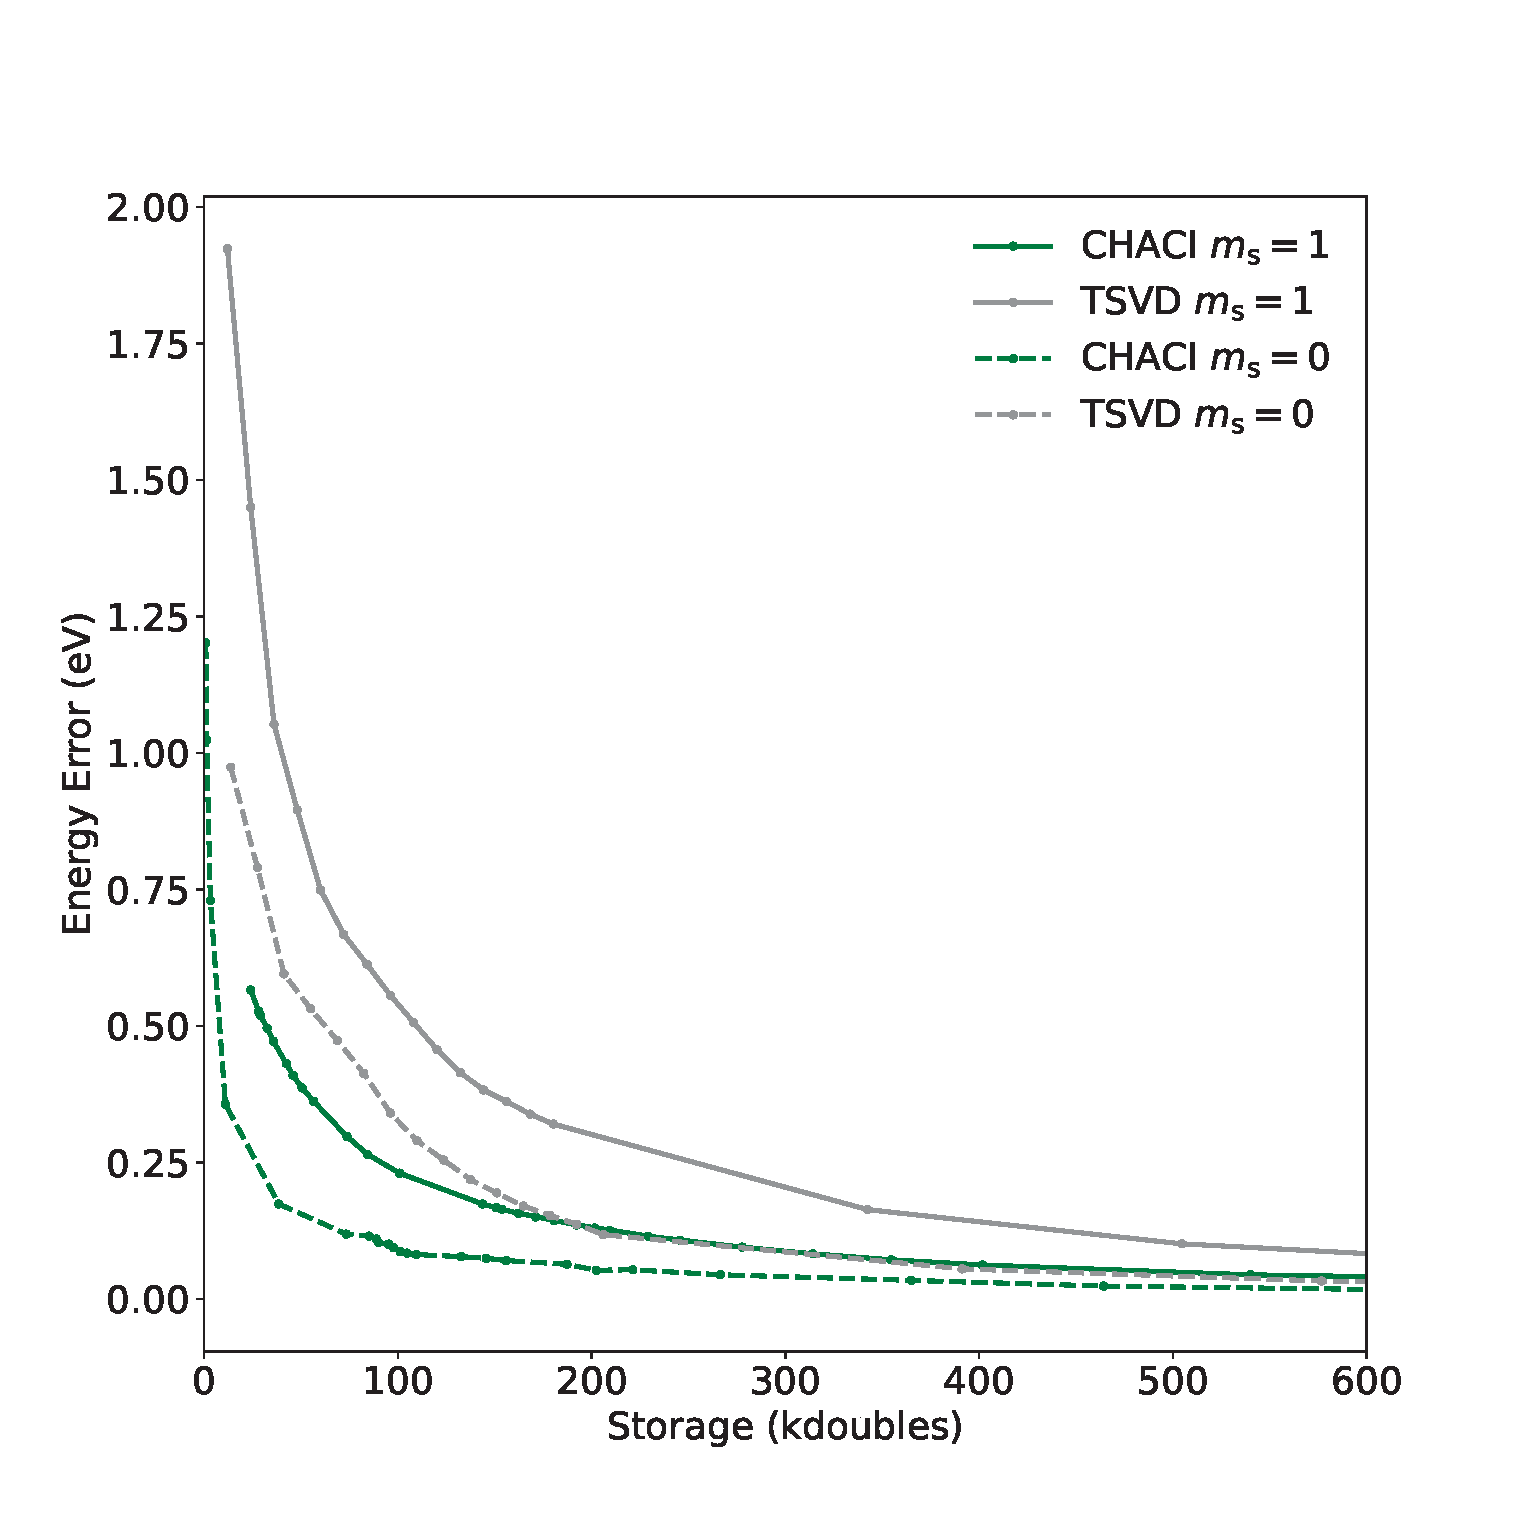
\includegraphics[width=0.5\linewidth]{figures/Degen_EN_Vs_St.eps}
    \caption{ The error in the absolute energies of two $m_s$ components of the triplet of 12-acene, computed with a 14-14 active space. Green and gray lines correspond to CHACI and TSVD, respectively.  Dashed and solid lines correspond to $m_s=0$ and $m_s=1$.}
    \label{fig:m_s_comparison-14-14}
\end{figure}

To investigate whether the convergence of states defined in different configuration spaces is balanced, we compare the convergence behavior of two rigorously degenerate states with very different CI vectors: the $m_s=0$ and $m_s=1$ components of the triplet (Fig. \ref{fig:m_s_comparison-14-14}).  The CHACI approach outperforms TSVD in all cases.  However, the $m_s=0$ wave function converges considerably more quickly with increasing storage than the $m_s=1$ wave function in both cases.  In addition, the discrepancy for CHACI is very large at some points, with the error in the absolute energy of the $m_s=1$ component being several times larger than that of the $m_s=0$ component.  This larger error is observed despite the fact that the $m_s=1$ CI vector is actually 24\% shorter than the $m_s=0$ vector.  It seems that achieving a balanced treatment of states defined in different configuration spaces is challenging.
}

\begin{figure}[htbp]
    \centering
    \includegraphics[width=0.6\linewidth]{figures/image6.eps}
    \caption{The error in the singlet-triplet gap of 12-acene as a function of total storage, computed with a 16-16 active space. The gray and green lines represent the error incurred by compression of the wave function using TSVD and CHACI, respectively.}
    \label{fig:error-gap-16-16}
\end{figure}

\begin{figure}[htbp]
    \centering
    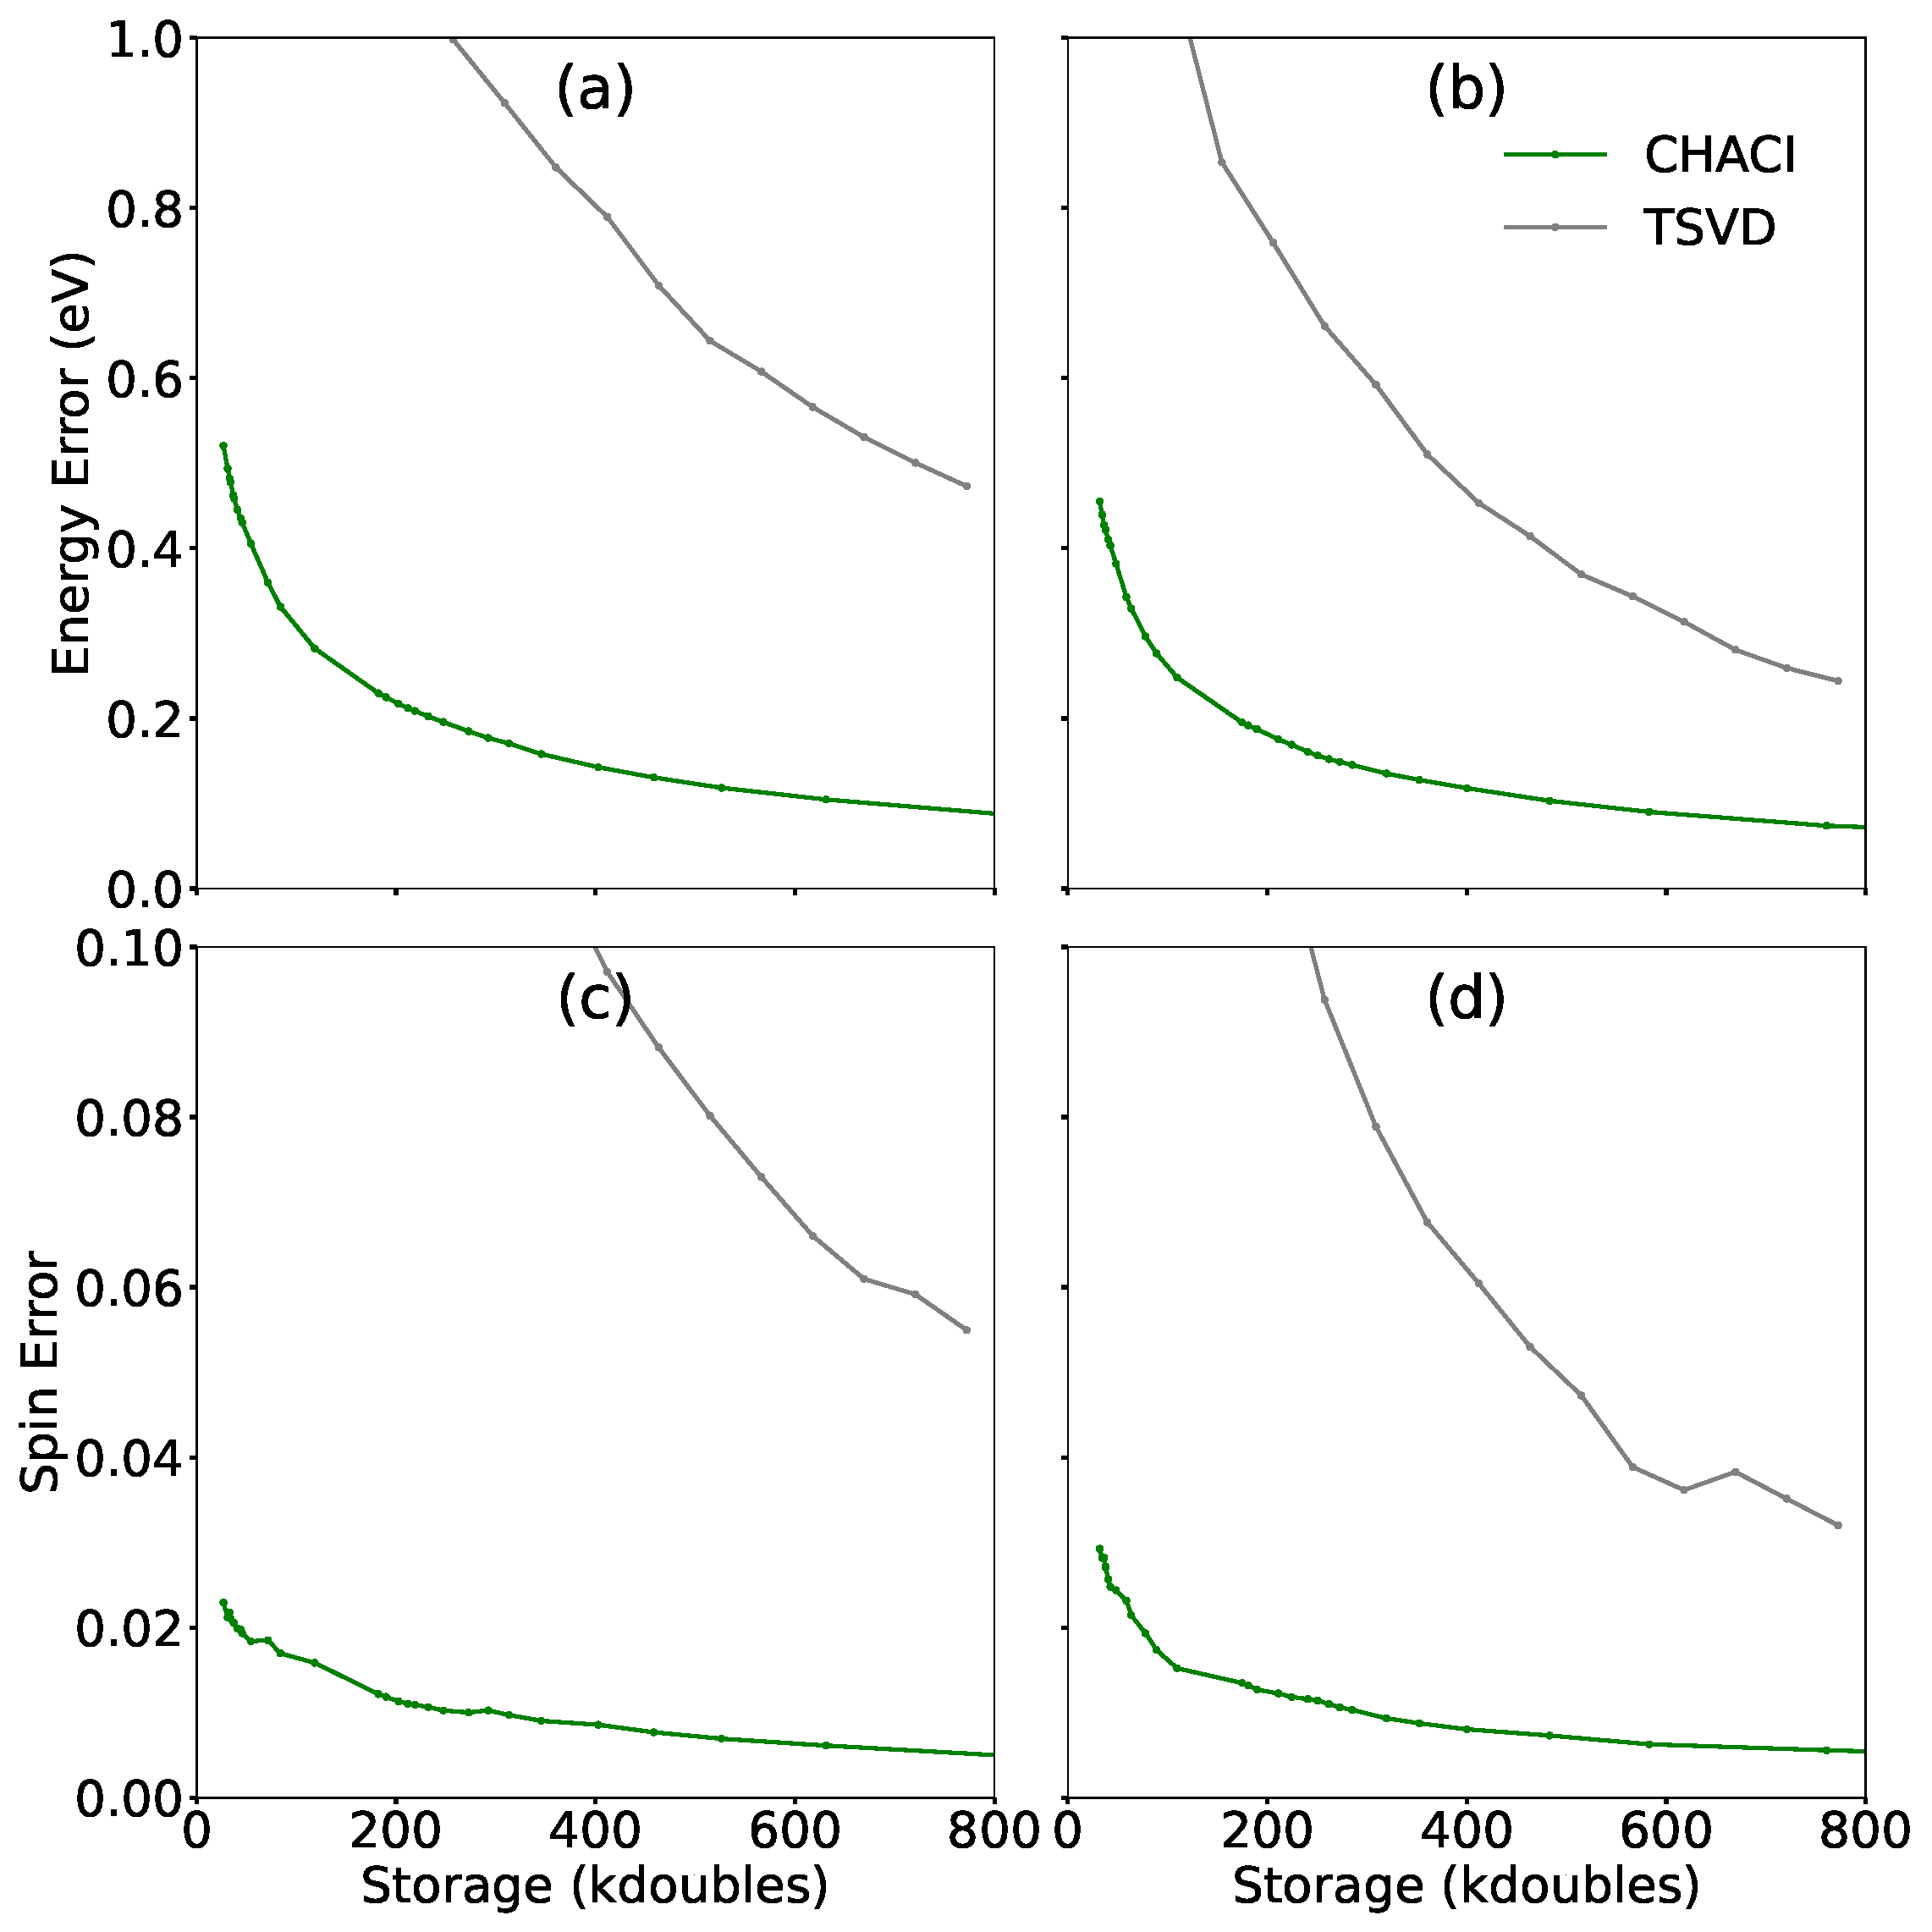
\includegraphics[width=6.50in, height=6.50in]{figures/image7.eps}
    \caption{Absolute energy (a and b) and spin (c and d) errors as a function of the storage for 12-acene with a 16-16 active space. Panel (a) and (c) correspond to the singlet wave function, while (b) and (d) correspond to the triplet wave function. The gray and green lines correspond to TSVD and CHACI compression, respectively.}
    \label{fig:energy-spin-errors-16-16}
\end{figure}

Figures~\ref{fig:error-gap-16-16} and \ref{fig:energy-spin-errors-16-16} demonstrate that the difference in performance between CHACI and TSVD increases when the active space size is increased from 14-14 to 16-16. In Figure~\ref{fig:error-gap-16-16}, it can be seen that errors in the singlet-triplet gap are at or below 0.1 eV for all cases, when CHACI is employed, even when only 59 kdoubles are stored (compared to 165,637 kdoubles for dense storage). Errors decrease rapidly with additional storage. In contrast, TSVD errors are above 0.2 eV for all cases. Similarly large differences in performance are observed for errors in absolute energy and spin in Figure~\ref{fig:energy-spin-errors-16-16}. As in the 14-14 case, CHACI does a much better job of maintaining the spin symmetry of the wave function than TSVD.

\subsection{Extrapolation of Performance to Larger Active Spaces}
\label{subsec:extrapolation-of-performance}
\begin{figure}[htbp]
    \centering
    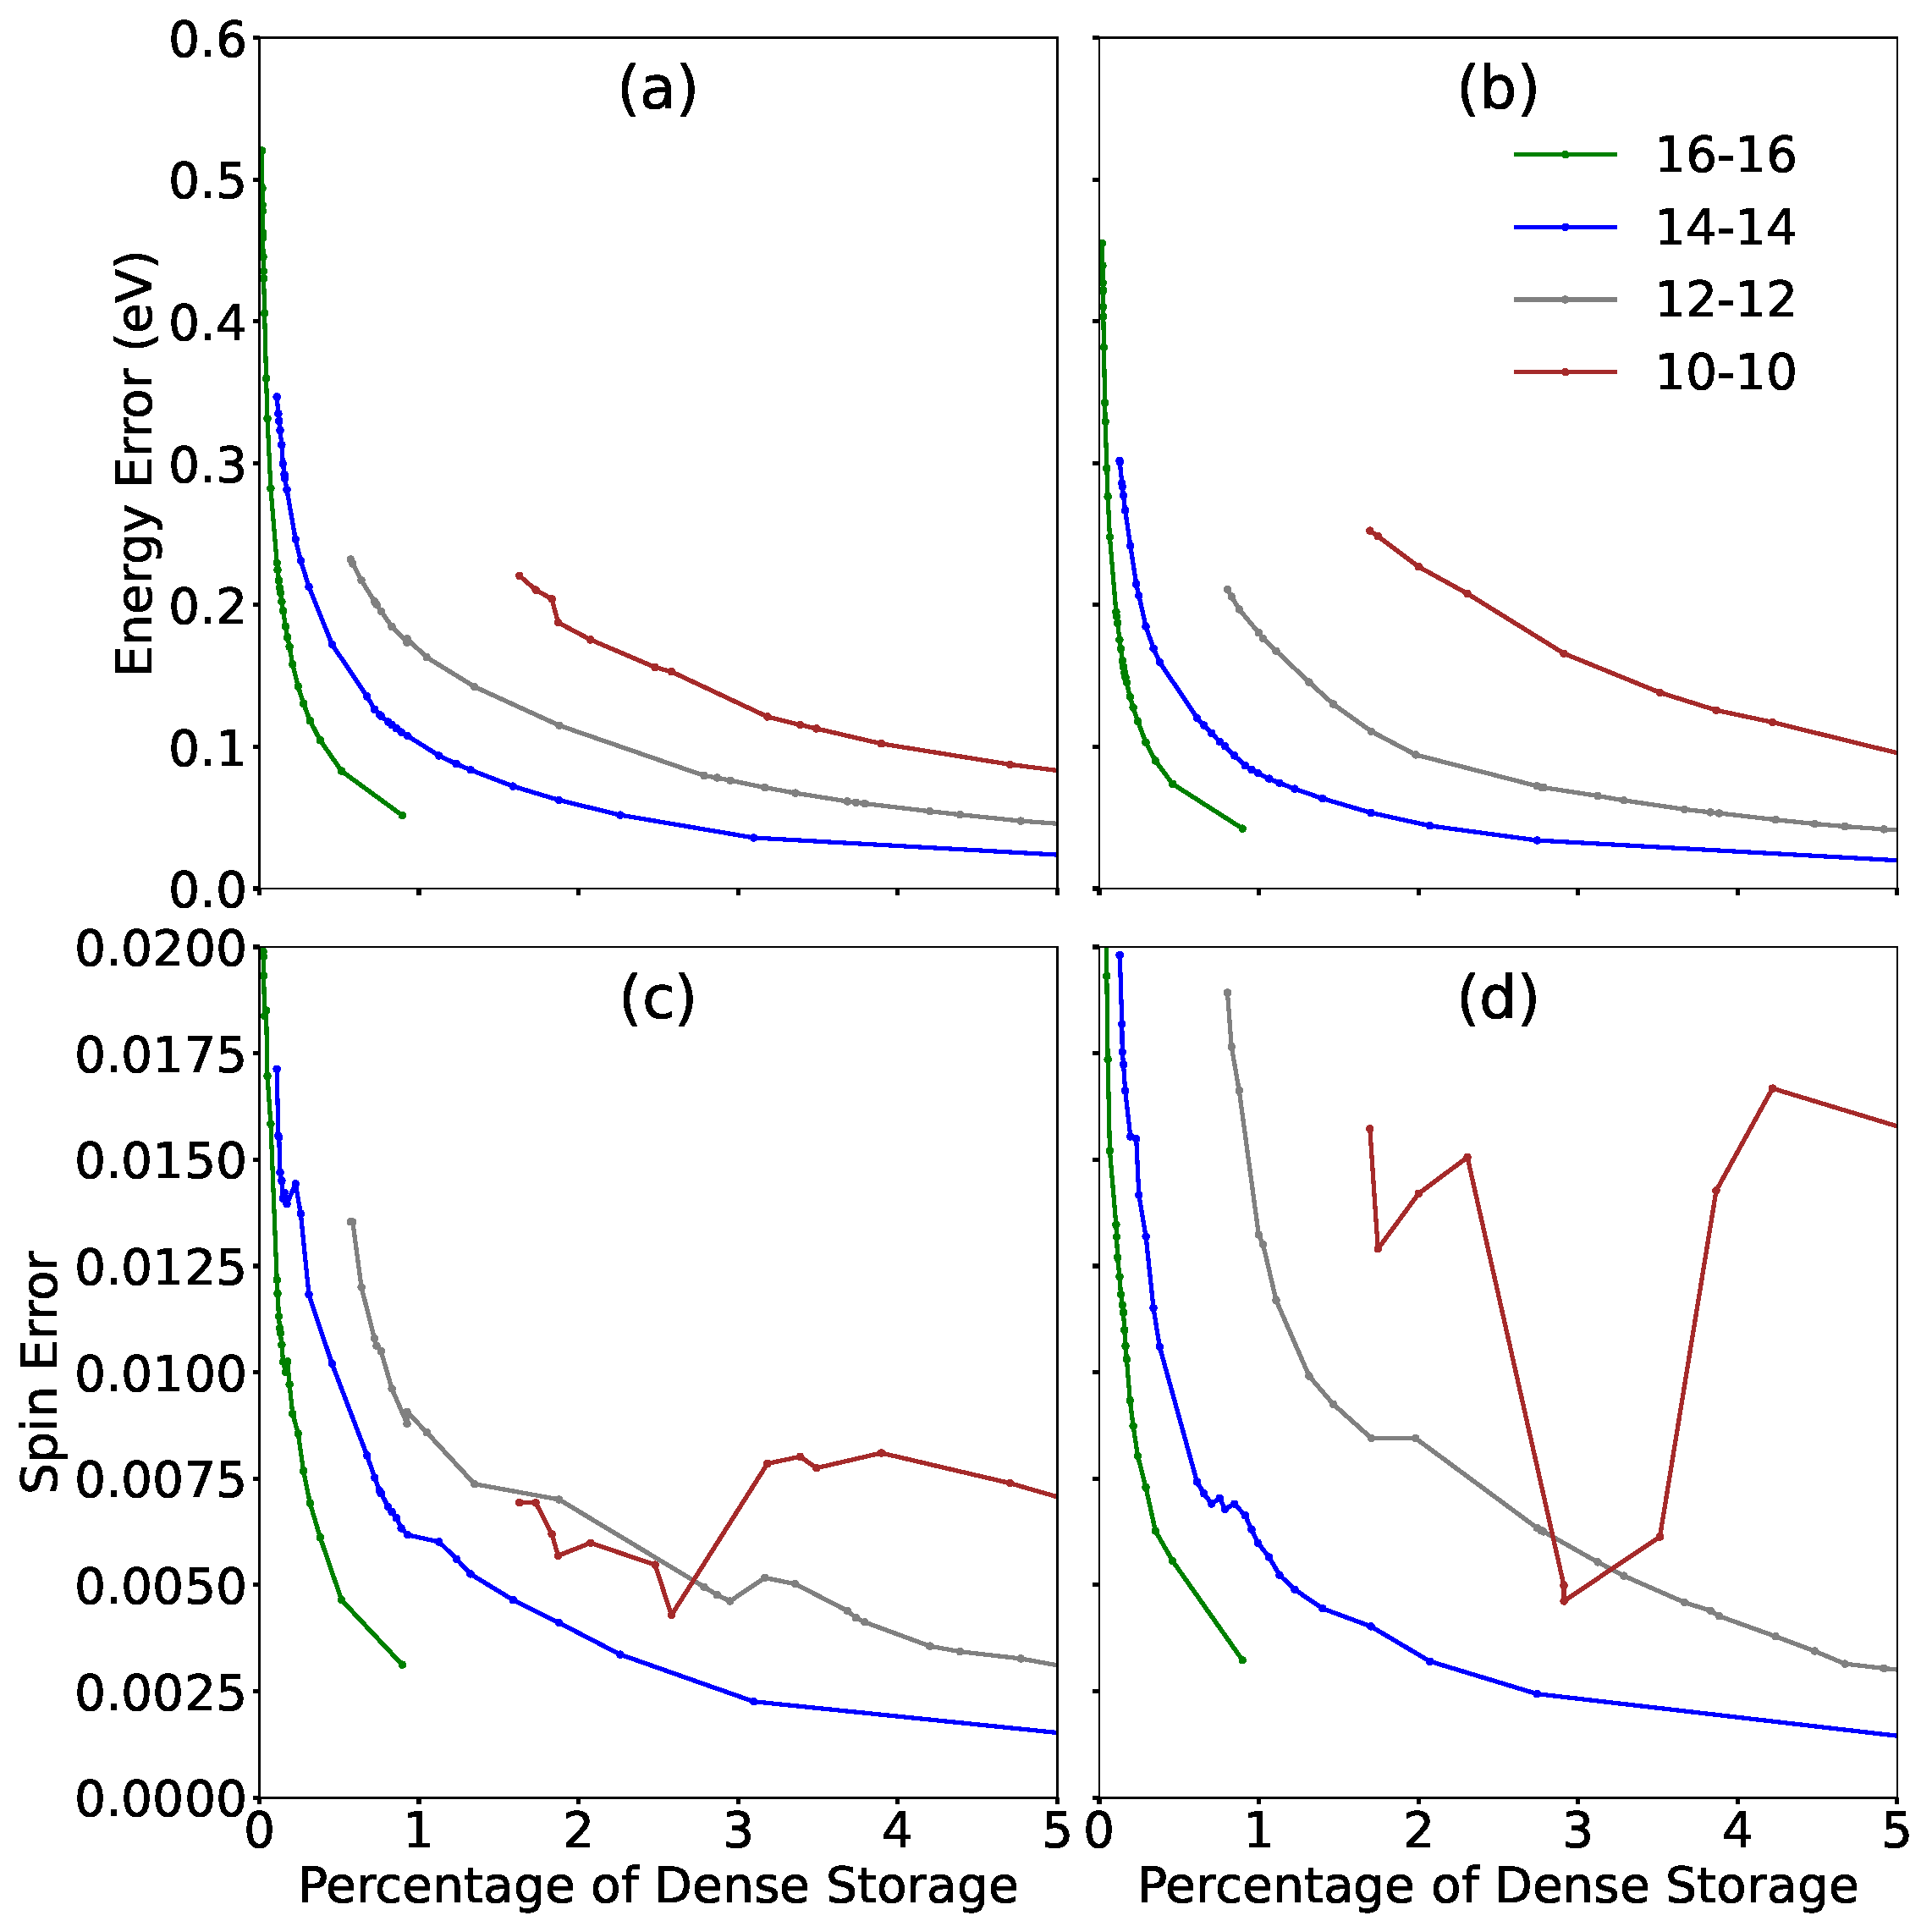
\includegraphics[width=5.89in, height=5.89in]{figures/image8.eps}
    \caption{The absolute energy (a and b) and spin errors (c and d) as a function of the percentage of dense storage for 12-acene with 10-10, 12-12, 14-14, and 16-16 active spaces. Panels (a) and (c) correspond to the singlet wave function, while panels (b) and (d) correspond to the triplet spin wave function.}
    \label{fig:errors-vs-compression-ratio}
\end{figure}

Ultimately, our goal is not to compute dense wave functions for subsequent compression. Our goal is to solve for large CI wave functions using a hierarchically compressed basis. Thus, in this section, we consider the behavior of CHACI compression as a function of active space size. In Figure~\ref{fig:errors-vs-compression-ratio}, we consider several active spaces, comparing the convergence of several measures of the accuracy as a function of the percentage of dense storage used (the compression ratio). We find that as the size of the active space increases, the accuracies of both absolute energy and spin converge faster with increasing compression ratio.

\begin{figure}[htbp]
    \centering
    \includegraphics[width=4.55in, height=4.45in]{figures/image9.eps}
    \caption{The storage ratio required to achieve \(<0.2\) eV accuracy in absolute energies as a function of the active space size. Blue and black lines correspond to the singlet and triplet wave functions, respectively.}
    \label{fig:compression-ratio-extrapolation}
\end{figure}

To quantify this convergence behavior, we plot the compression ratio at which absolute energies of 0.2 eV accuracy are achieved as a function of the number of active orbitals/electrons in Figure~\ref{fig:compression-ratio-extrapolation}. Both the singlet and triplet compression ratios converge quickly with increasing active space. Of the two, the triplet energy converges more slowly, thus we fit it to an exponential in order to extrapolate to larger active spaces. We find that the required compression ratio decays proportional to
\begin{equation}
f(N_\text{MO}) \propto e^{-0.561N_\text{MO}}.
\end{equation}
Extrapolating to larger active spaces, we estimate that a 24-24 active space could converge to 0.2 eV accuracy at a storage cost of 77,370 kdoubles, which is less than the cost of the dense storage of a 16-16 active space (165,637 kdoubles). Though the convergence behavior is likely to be system-dependent, this result certainly encourages further study.

{
\subsection{Effect of Compression on the Potential Energy Surface}
\label{subsec:effect-of-compression-on-the-pes}
\begin{figure}[htbp]
    \centering
    \includegraphics[height=4.0in]{figures/Singlet_PES.pdf}
    \caption{The PES of 12-acene as a function of the displacement of a single carbon atom out of plane, computed with a 14-14 active space.  Results in the low, medium, and high storage regimes ($\sim$50, $\sim$130, $\sim$190 kdoubles) are compared to exact CASCI results.}
    \label{fig:pes}
\end{figure}

It is interesting to consider how a potential energy surface (PES) is effected by compression for two reasons.  First, one might expect that compression might introduce non-parallelity error.  Second, as one moves from point to point along the PES, one might expect discontinuities as specific singular vector pairs are added or dropped.  

To investigate this possibility, we have computed the PES as a function of the out-of-plane displacement of a single carbon atom in 12-acene in three different storage regimes (Fig. \ref{fig:pes}).  No discontinuities are observed on the scale of 0.01 eV in any of the plots.  Comparing the energies at the first and last points of each curve, we observe very small deviations from parallelity: $5\times10^{-4}$, $3\times10^{-4}$, and $4\times10^{-5}$ eV in the low, medium, and high storage regimes, respectively.
}

\subsection{Effect of Using Optimal Rank on Compression}
\label{subsec:effect-of-dynamic-rank-on-compression}
\begin{figure}[htbp]
    \centering
    \includegraphics[width=6.41in, height=4.49in]{figures/image10.eps}
    \caption{The SR-CHACI error (blue) in the singlet-triplet gap of 12-acene as a function of total storage, computed with a 14-14 active space. The TSVD and CHACI errors (gray and green, respectively) are shown for comparison.}
    \label{fig:SR-CHACI-gap-error}
\end{figure}

In order to assess the necessity of the optimal rank procedure, we compare SR-CHACI (which uses a static rank) to CHACI and TSVD. Figure~\ref{fig:SR-CHACI-gap-error} presents the error in the singlet-triplet gap as a function of the total storage for the 14-14 active space. Excepting one fortunate point at 160 kdoubles, the accuracy of SR-CHACI is significantly worse than that of CHACI, but still better than TSVD. However, considering the error in the absolute energies of the singlet and triplet states separately (Figure 11a and b, respectively), it is clear that this is due to error cancellation. Errors in the absolute energy of the singlet state derived from the SR-CHACI wave function are similar to those of TSVD, and much greater than those of CHACI. Further, errors in the SR-CHACI triplet state are slightly larger than TSVD.

\begin{figure}[htbp]
    \centering
    \includegraphics[width=6.50in, height=6.50in]{figures/image11.eps}
    \caption{The SR-CHACI errors (blue) in the absolute energy (a and b) and spin (c and d) as a function of the storage for 12-acene (14-14 active space). Panels (a) and (c) correspond to the singlet wave function, while (b) and (d) correspond to the triplet wave function. The TSVD (gray) and CHACI (green) errors are shown for comparison.}
    \label{fig:SR-CHACI-energy-spin-errors}
\end{figure}

Analysis of spin errors tells a similar story. CHACI is much superior to SR-CHACI at reproducing the spin of the original wave function, and SR-CHACI has similar (and sometimes larger) spin errors compared to TSVD. Taken together, we conclude that optimal rank is an essential component of the CHACI algorithm.

\subsection{Effect of Sorting on Compression}
\label{subsec:effect-of-sorting-on-compression}
Here we assess the necessity of another feature of the CHACI compression algorithm: the sorting of rows/columns of the \(\mathbf{C}\) matrix prior to compression. To this end, we compare U-CHACI, in which the rows/columns remain unsorted, to CHACI and TSVD. Figure~\ref{fig:CI-vector-heatmap} presents a heat-map of the uncompressed \(\mathbf{C}\) matrix of the singlet (panels a and c) and triplet (b and d) wave functions before (a and b) and after (c and d) sorting. Note that sorting concentrates larger elements into the upper-left corner of the matrix.

\begin{figure}[htbp]
    \centering
    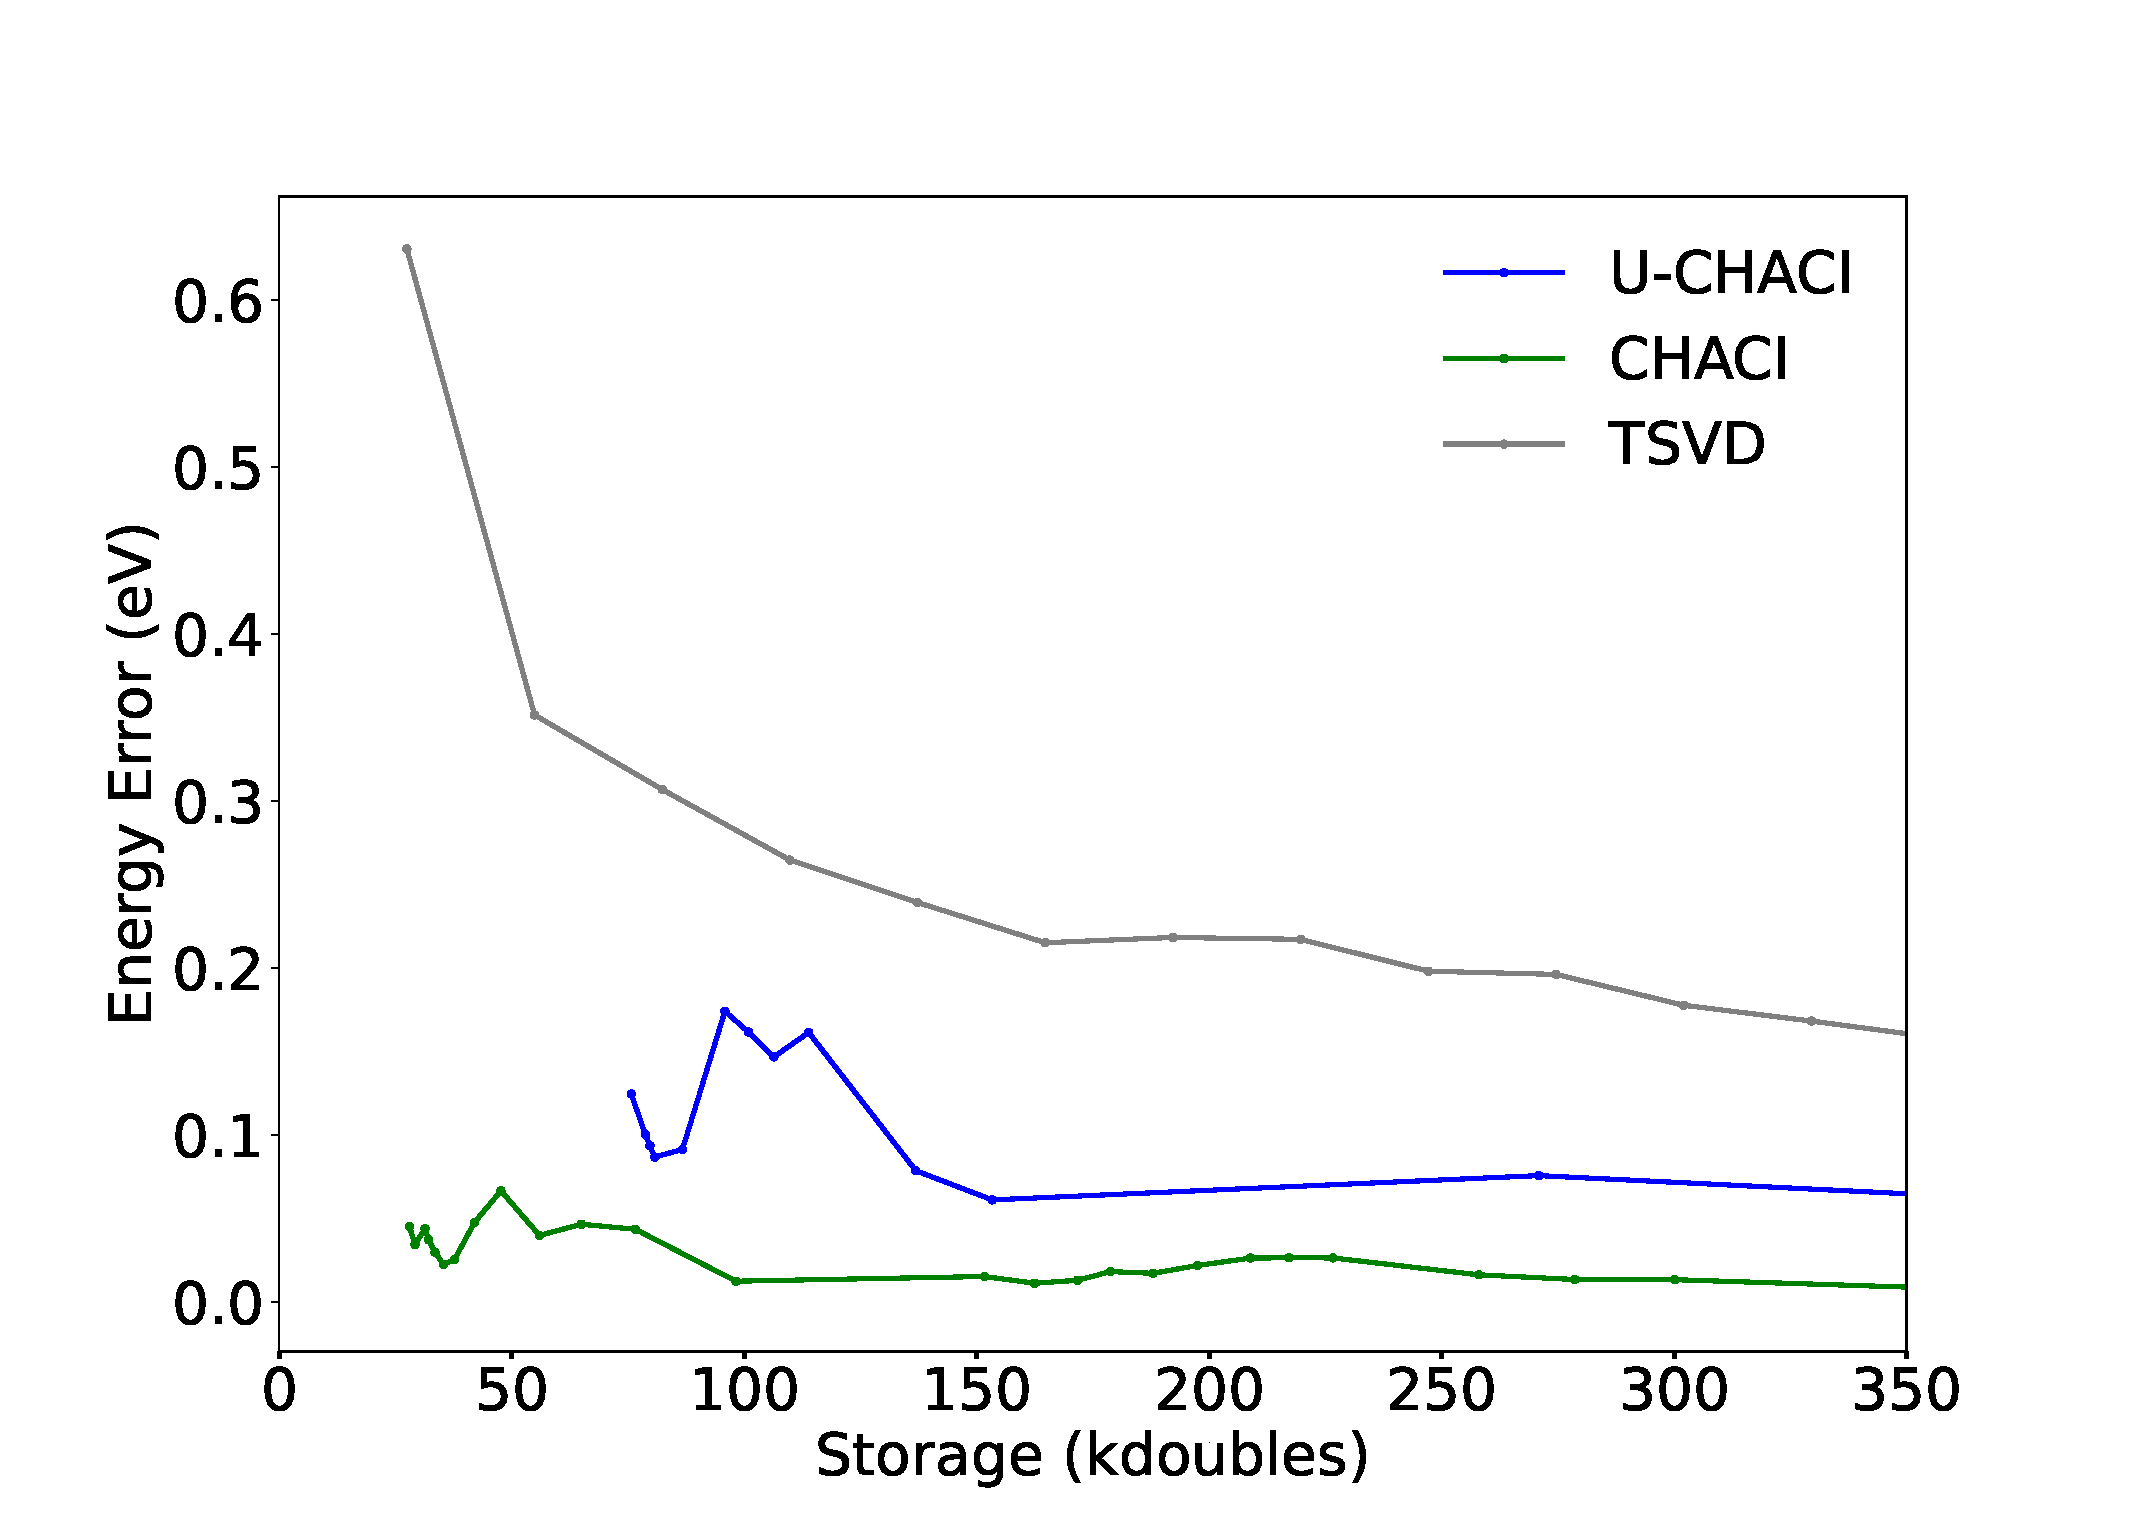
\includegraphics[width=4.59in, height=3.22in]{figures/image13.eps}
    \caption{The U-CHACI error (blue) in the singlet-triplet gap of 12-acene as a function of total storage, computed with a 14-14 active space. The TSVD and CHACI errors (gray and green, respectively) are shown for comparison.}
    \label{fig:U-CHACI-gap-error}
\end{figure}

Figure~\ref{fig:U-CHACI-gap-error} compares the U-CHACI singlet-triplet errors to those of CHACI and TSVD. Though U-CHACI appears to be more accurate for predicting the relative energy than TSVD, it remains inferior to CHACI. Considering the errors in the absolute singlet and triplet energies (Figure~\ref{fig:SR-CHACI-energy-spin-errors}a and b), we see that U-CHACI errors are on the order of the same size as those of TSVD, and considerably larger than those of CHACI. That being said, U-CHACI is solidly between CHACI and TSVD in its ability to accurately describe the total spin angular momentum (Figure~\ref{fig:SR-CHACI-energy-spin-errors}c and d).

\begin{figure}[htbp]
    \centering
    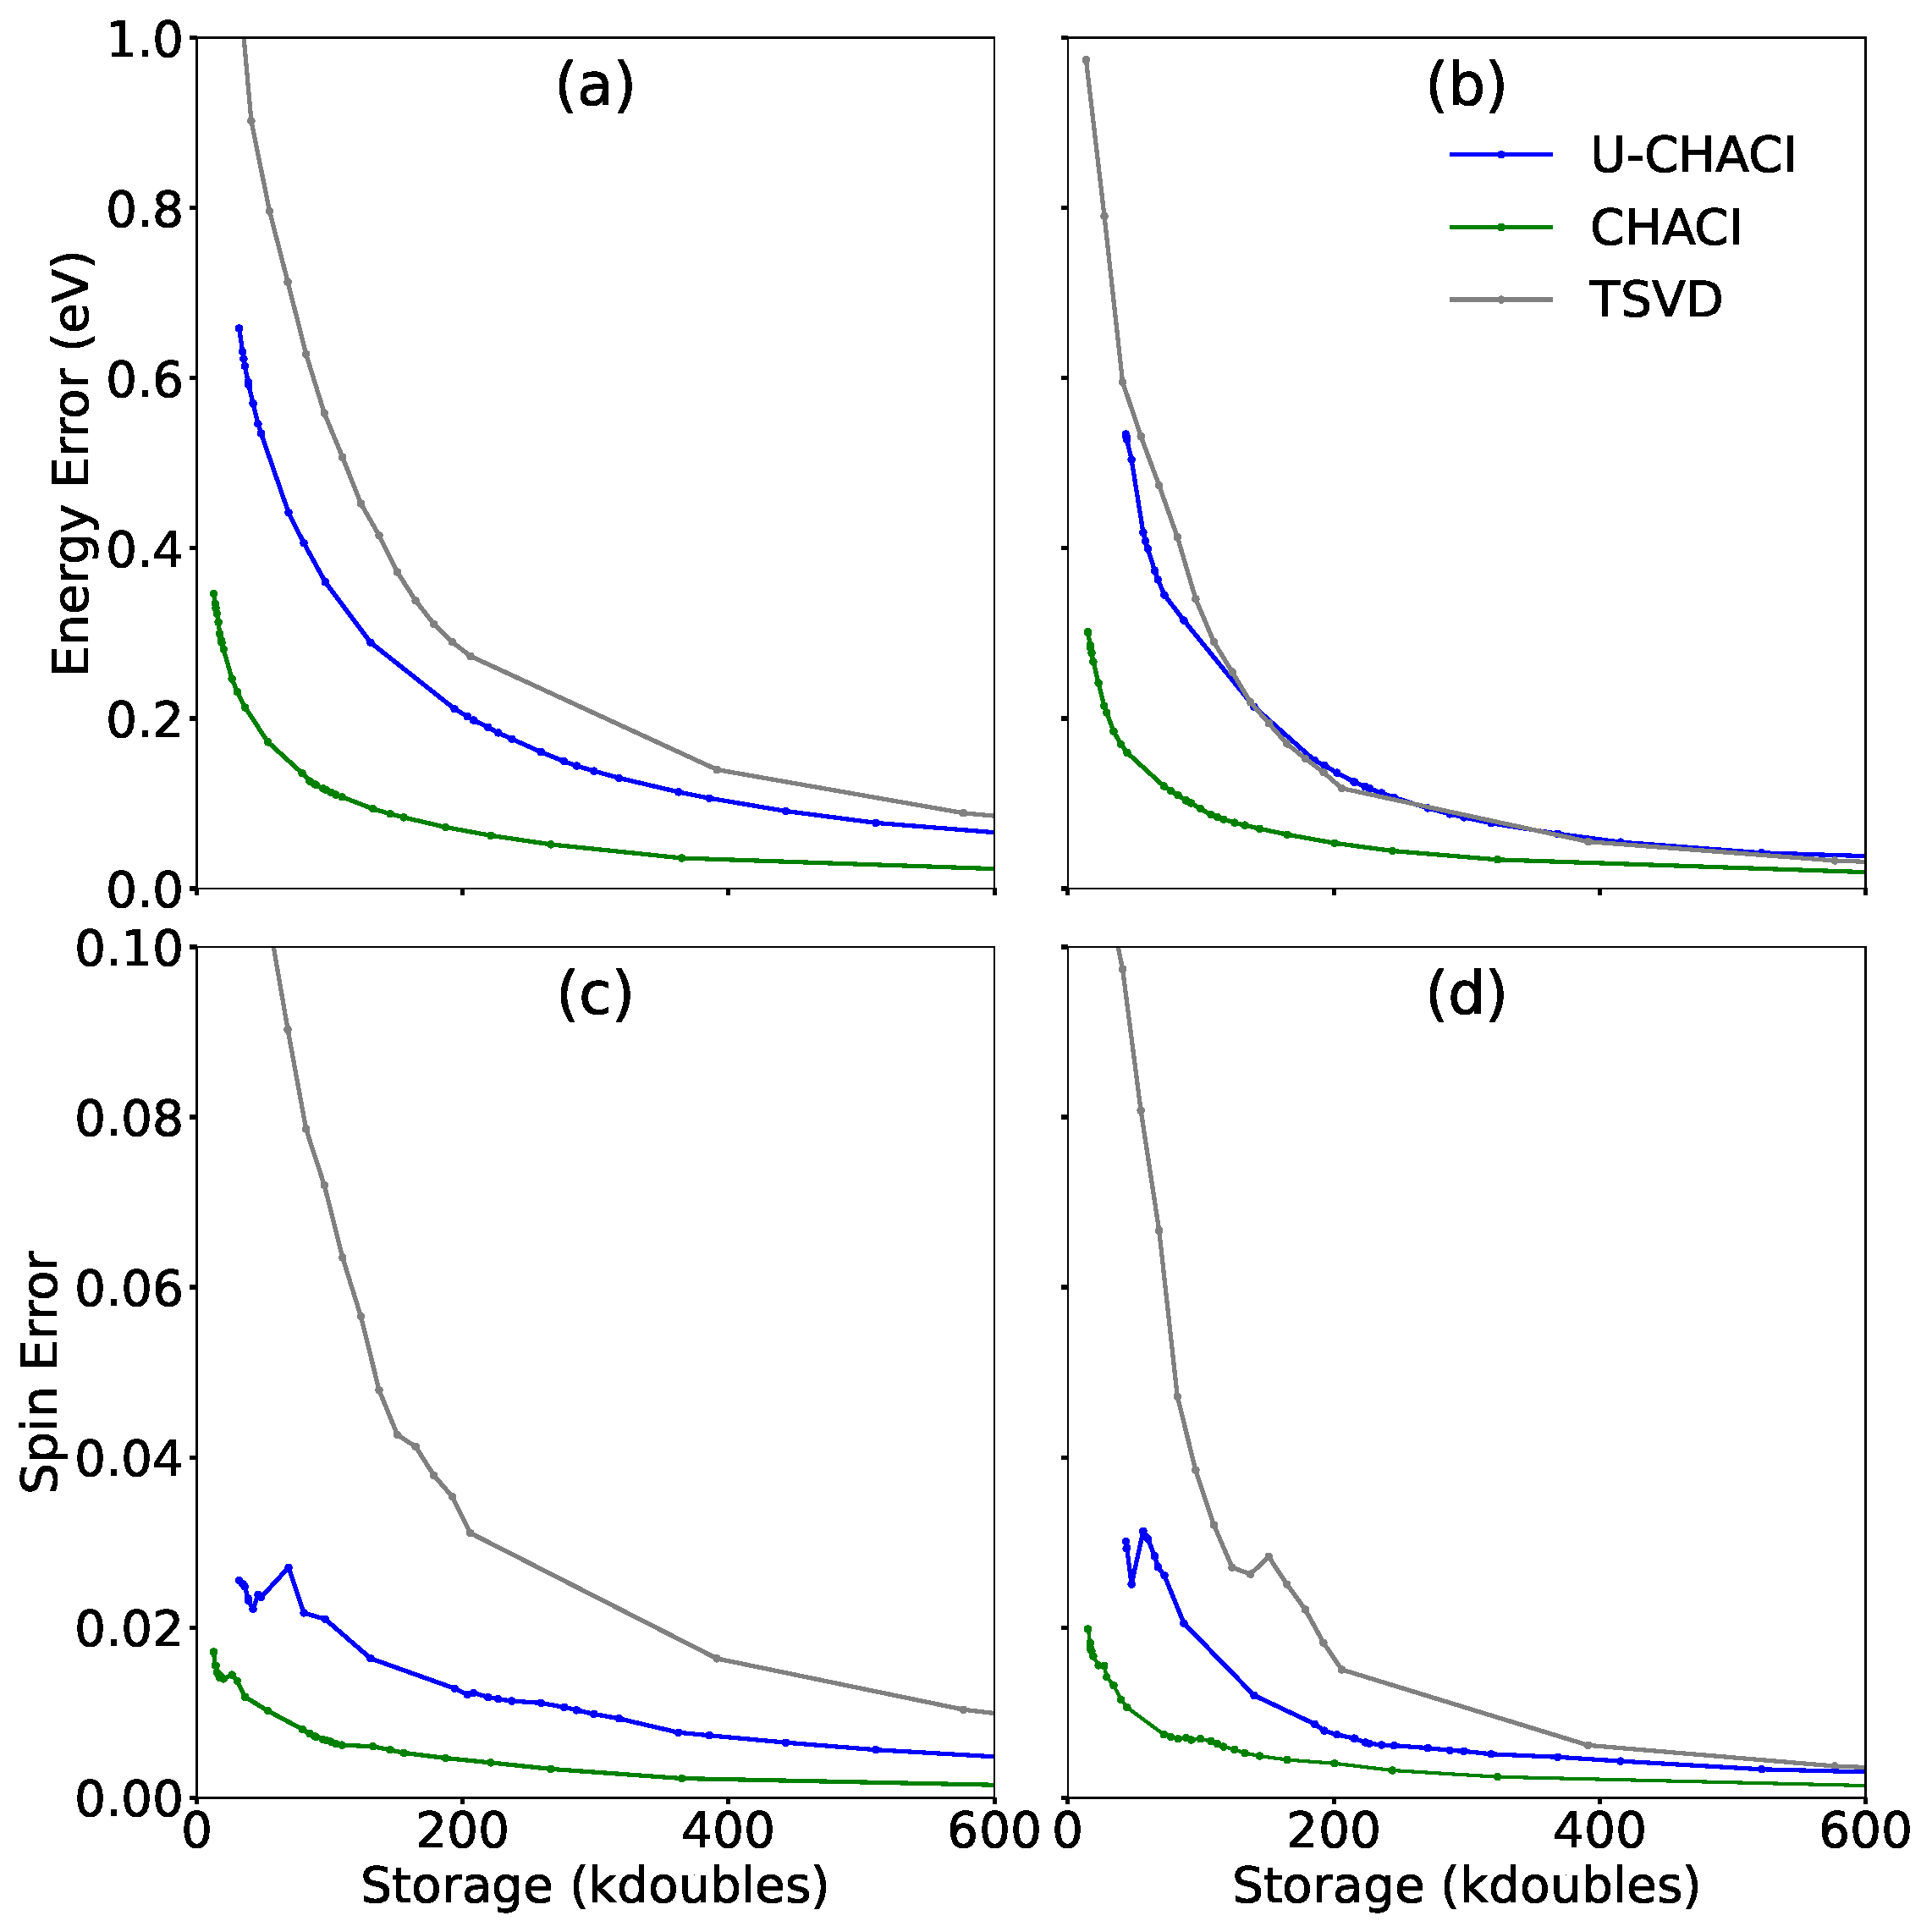
\includegraphics[width=4.26in, height=4.26in]{figures/image14.eps}
    \caption{The U-CHACI errors (blue) in the absolute energy (a and b) and spin (c and d) errors as a function of the storage for 12-acene (14-14 active space). Panels (a) and (c) correspond to the singlet wave function, while (b) and (d) correspond to the triplet wave function. The TSVD (gray) and CHACI (green) errors are shown for comparison.}
    \label{fig:U-CHACI-energy-spin-errors}
\end{figure}

Taking this data together, we conclude that sorting is an essential component of the CHACI algorithm. However, our ultimate goal is not to compute the full wave function and subsequently compress it, and the type of \textit{a posteriori} sorting that we use in CHACI would not be possible if we were to directly solve for the wave function in compressed form. But given that the Duch ordering of spin strings does not allow for efficient compression, the determination of an \textit{a priori} scheme by which strings may be ordered for efficient compression remains an important open question.

\subsection{Effect of Upper Quadrant vs H-matrix Compression}
\label{subsec:effect-of-upper-quadrant}
\begin{figure}[htbp]
    \centering
    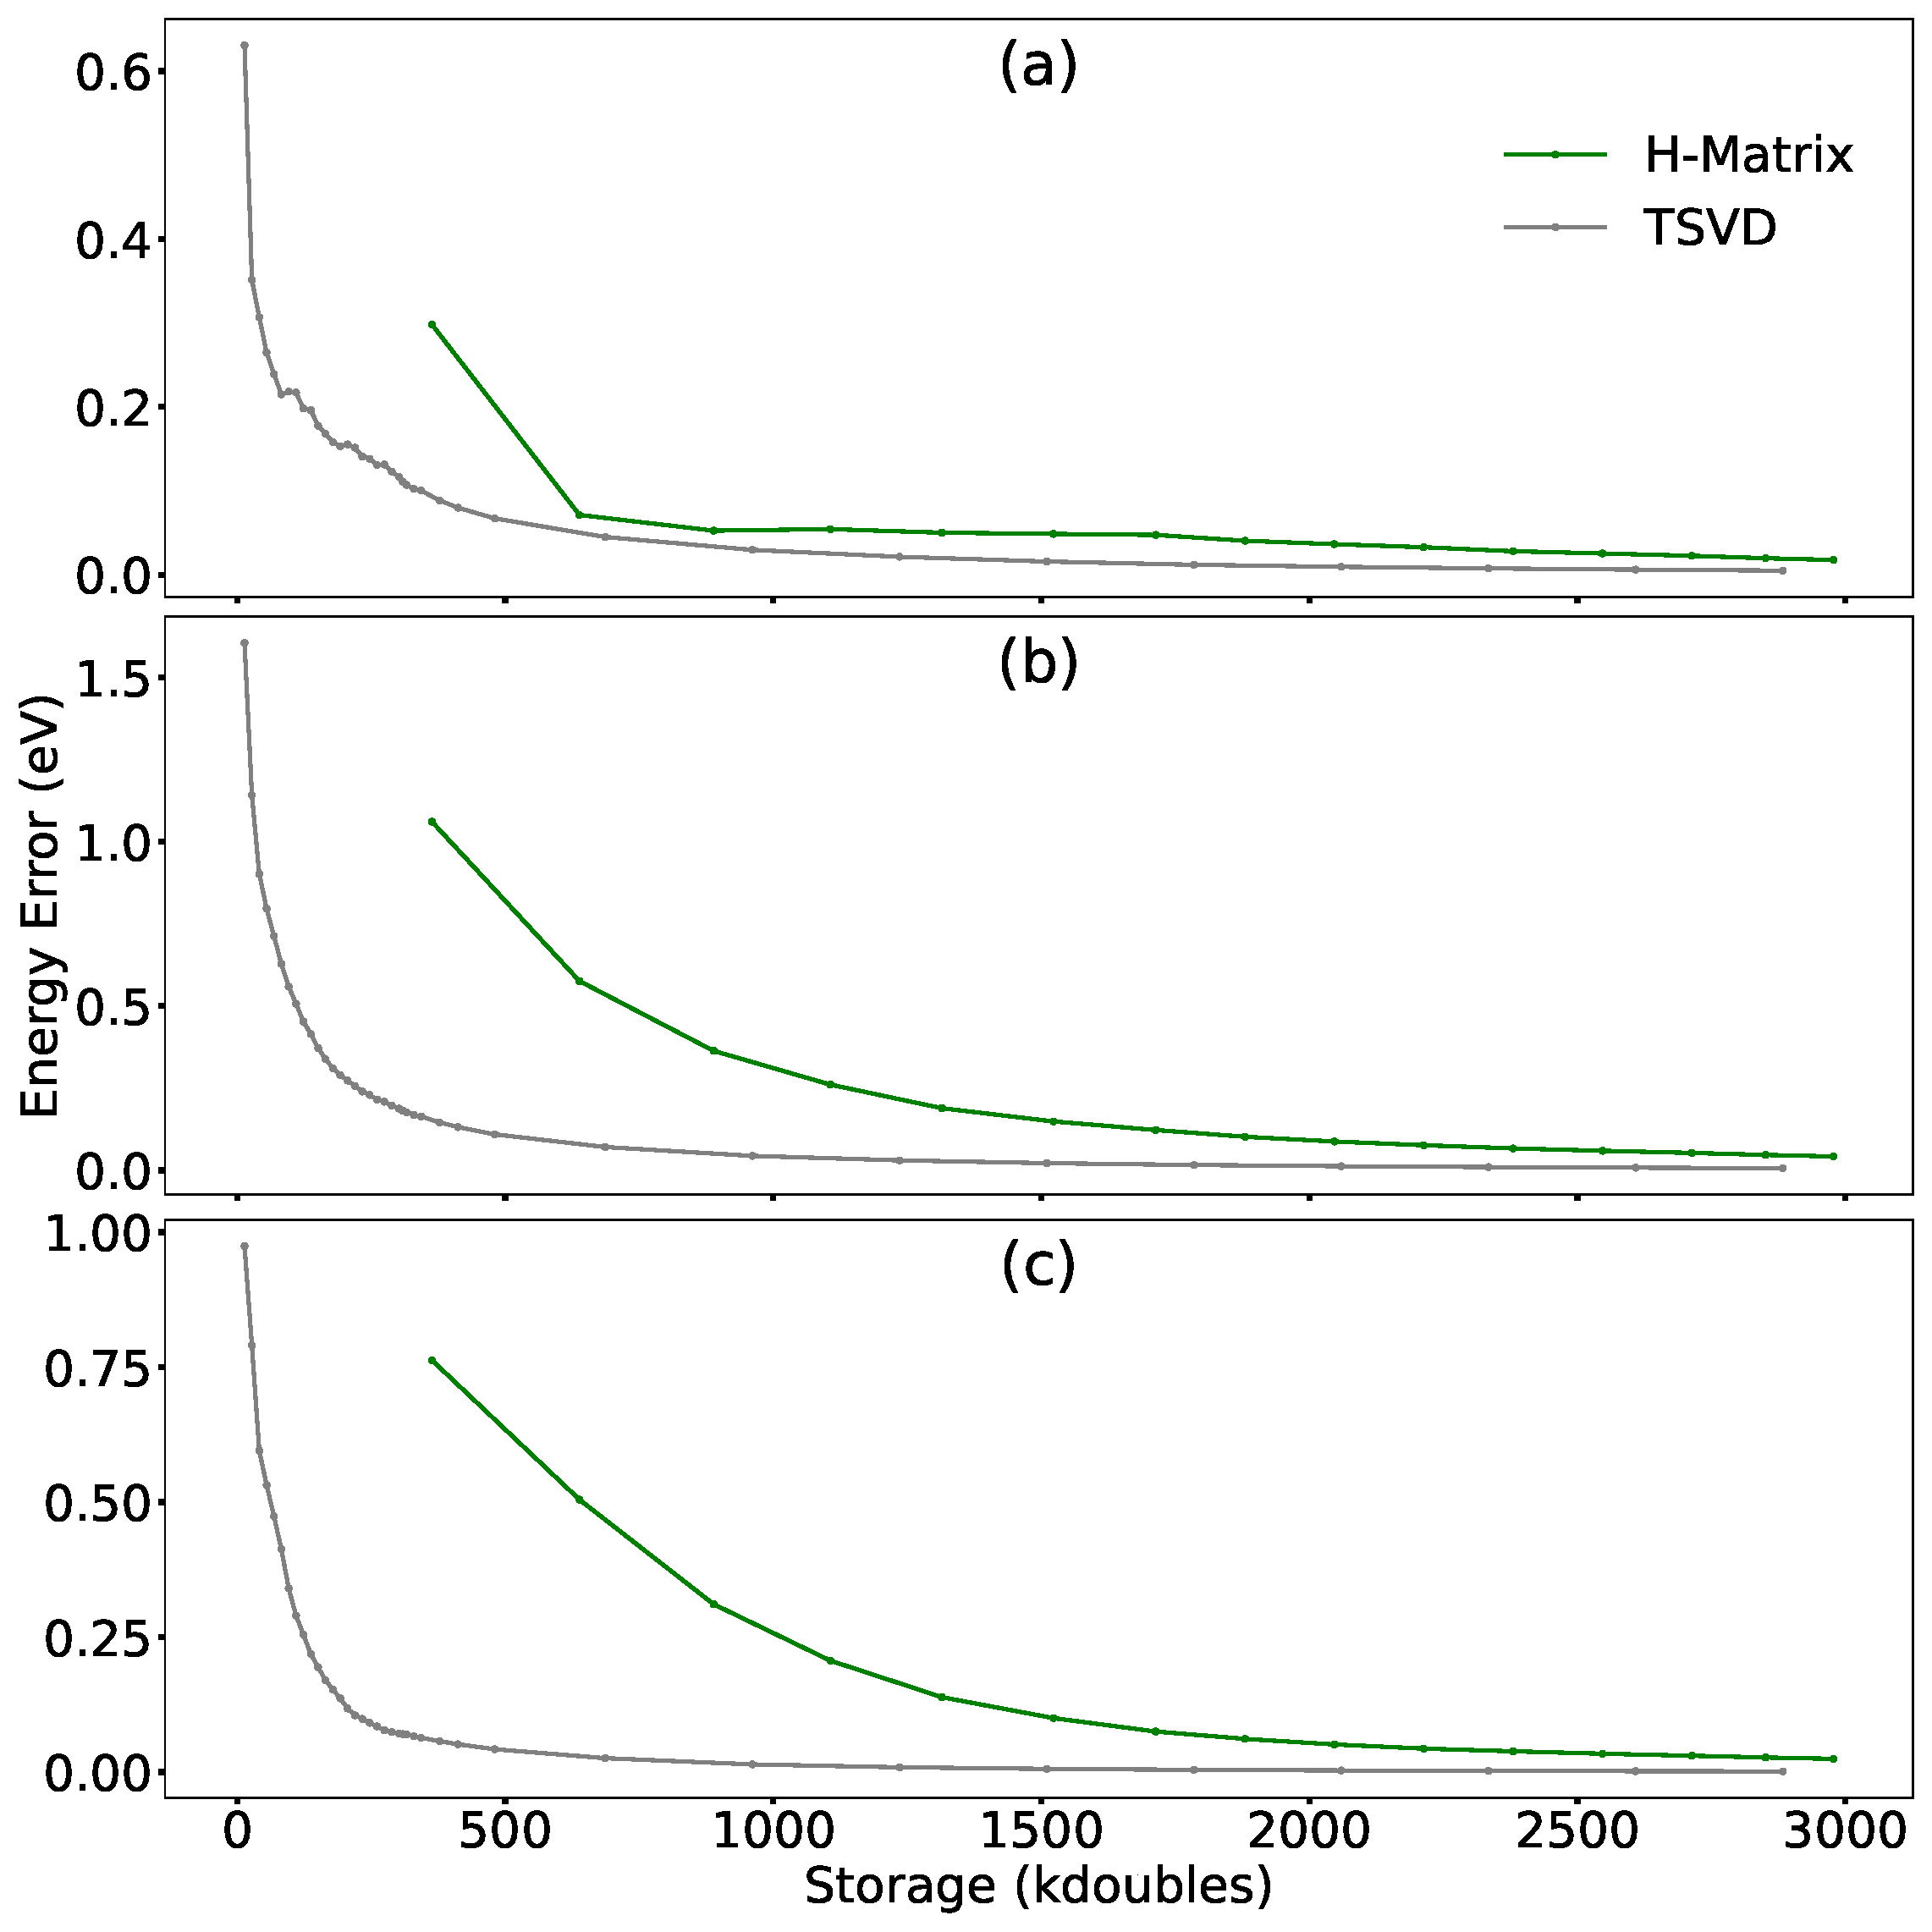
\includegraphics[width=4.79in, height=4.79in]{figures/H-Matrix.eps}
    \caption{Panels (a), (b), and (c) show the errors in the singlet-triplet gap, singlet, and triplet energies, respectively, of 12-acene (14-14 active space) as a function of the required storage for H-matrix and TSVD compression (green and gray).}
    \label{fig:H-matrix-vs-SVD}
\end{figure}

Lastly, we consider compression of \(\mathbf{C}\) into the H-matrix format,\cite{Hackbusch1999} which is designed to leverage the diagonally dominant nature of the matrix, in contrast to the CH blocking scheme used in CHACI. Figure~\ref{fig:H-matrix-vs-SVD} shows the error in the singlet-triplet gap, singlet absolute energy, and triplet absolute energy of the 14-14 wave function compressed into H-matrix format. H-matrix compression is inferior to TSVD, thus we conclude that the CH blocking scheme is an essential component of the CHACI scheme.
\chapter{Hierarchically Compressed SOS-MP2 Algorithm}
\label{chap:h2mp2}

In this chapter we describe a hierarchically compressed spin-opposite-scaled
(SOS-) MP2 algorithm based on the work of Gao, Jiao, and
Levine~\cite{GaoJiaoLevineH2MP2}. The method combines the atomic-orbital
(AO) Laplace-transformed formulation of the MP2 energy with an $\mathcal{H}^2$
representation of the electron repulsion integral (ERI) tensor. The key idea is
to exploit both the data-sparsity of the ERI tensor in $\mathcal{H}^2$ form and
the element-wise sparsity of the energy-weighted density and complementary
density matrices.

\section{From closed-shell MP2 to the AO--Laplace trace form}
\label{sec:AOLaplaceMP2_trace}

We outline the algebraic steps that lead from the conventional closed-shell MP2
energy expression to an AO--Laplace formulation that can be evaluated via
trace contractions. This derivation provides the analytic target that the
hierarchical algorithm in Algorithm~\ref{alg:HSM algorithm} accelerates.

\paragraph{Closed-shell MP2 energy.}
In canonical molecular orbitals (MOs), the closed-shell MP2 correlation energy
may be written as
\begin{equation}
E_{\mathrm{MP2}}
=
-\sum_{ij}^{\mathrm{occ}}\sum_{ab}^{\mathrm{vir}}
\frac{(ia|jb)\,\bigl[2(ia|jb)-(ib|ja)\bigr]}
{\epsilon_a+\epsilon_b-\epsilon_i-\epsilon_j},
\label{eq:mp2_closed_shell}
\end{equation}
where \((pq|rs)\) are two-electron repulsion integrals (ERIs) in chemists'
notation and \(\Delta_{ij}^{ab}=\epsilon_a+\epsilon_b-\epsilon_i-\epsilon_j>0\)
denotes the orbital energy gap.

\paragraph{Laplace transform and quadrature.}
Using the Laplace identity \(1/\Delta=\int_0^\infty e^{-\Delta t}\,dt\) and a
quadrature approximation with \(\{t_\alpha,w_\alpha\}_{\alpha=1}^{n_q}\), we obtain
\begin{equation}
E_{\mathrm{MP2}}
\approx
\sum_{\alpha=1}^{n_q} w_\alpha\, e_2^\alpha,
\qquad
e_2^\alpha
=
-\sum_{ijab}
(ia|jb)\,\bigl[2(ia|jb)-(ib|ja)\bigr]\,
e^{-\Delta_{ij}^{ab}t_\alpha}.
\label{eq:mp2_laplace_quadrature}
\end{equation}
Since \(e^{-\Delta_{ij}^{ab}t_\alpha}
=
e^{+\epsilon_it_\alpha}e^{+\epsilon_jt_\alpha}e^{-\epsilon_at_\alpha}e^{-\epsilon_bt_\alpha}\),
we define at each quadrature point \(\alpha\) the energy-weighted density and
complementary density matrices in the AO basis,
\begin{align}
X_{\mu\nu}^{\alpha}
&=
\sum_{i}^{\mathrm{occ}} C_{\mu i}C_{\nu i}\,e^{+\epsilon_i t_\alpha},
\label{eq:X_def_trace}
\\
Y_{\mu\nu}^{\alpha}
&=
\sum_{a}^{\mathrm{vir}} C_{\mu a}C_{\nu a}\,e^{-\epsilon_a t_\alpha},
\label{eq:Y_def_trace}
\end{align}
where \(C\) denotes the MO coefficient matrix.

\paragraph{AO formulation via index-transformed ERIs.}
Let \(W\) denote the AO ERI tensor \(W_{\mu\nu\lambda\sigma}\equiv(\mu\nu|\lambda\sigma)\).
After applying the Laplace transform and quadrature, the MP2 energy becomes a weighted sum over quadrature points. In the remainder of this section we fix \emph{one} quadrature point and, for notational simplicity, drop the quadrature index \(\alpha\) on all quantities (i.e., \(X\equiv X^\alpha\), \(Y\equiv Y^\alpha\), etc.).

At the chosen quadrature point, the Laplace factors are absorbed into the energy-weighted density matrix \(X\) and complementary density matrix \(Y\) (Eq. ~\eqref{eq:X_def_trace}--\eqref{eq:Y_def_trace}). In the notation used
throughout this chapter and in Algorithm~\ref{alg:HSM algorithm}, we perform two
successive \emph{ket-side} index transformations:
\begin{align}
(\mu\nu|\underline{\lambda}\epsilon)
&\equiv
\sum_{\kappa}(\mu\nu|\kappa\epsilon)\,X_{\kappa\lambda},
\label{eq:half_transform_unified}
\\
(\mu\nu|\underline{\lambda}\overline{\sigma})
&\equiv
\sum_{\epsilon}(\mu\nu|\underline{\lambda}\epsilon)\,Y_{\epsilon\sigma}.
\label{eq:full_transform_unified}
\end{align}
Here \(\underline{\lambda}\) and \(\overline{\sigma}\) indicate transformed (and, in
practice, threshold-truncated) indices induced by \(X\) and \(Y\), respectively.

Define the Kronecker product
\begin{equation}
Z \equiv X\otimes Y,
\label{eq:Z_def_unified}
\end{equation}
which acts on the \emph{column} (ket) pair index \((\lambda\sigma)\), and the one-sided
index-transformed ERI matrix
\begin{equation}
T \equiv W Z,
\qquad
T_{(\mu\nu),(\lambda\sigma)} \equiv (\mu\nu|\underline{\lambda}\overline{\sigma}).
\label{eq:T_def_unified}
\end{equation}
The fully index transformed ERI matrix is then expressed as
\begin{equation}
Q \equiv Z W Z.
\label{eq:Q_def_unified}
\end{equation}

With these definitions, the MP2 contribution can be written as two
trace contractions: a Coulomb contraction with \(W\) and an exchange contraction with a
permuted ERI matrix \(V\) whose entries are \(V_{(\mu\nu),(\lambda\sigma)}=(\mu\sigma|\lambda\nu)\),
i.e., \(V=\Pi(W)\) for a fixed permutation \(\Pi\) on pair indices,
\begin{equation}
e_2
=
-2\,\mathrm{Tr}(Q W)
\;+\;
\mathrm{Tr}(Q V).
\label{eq:e2_trace_two_terms_unified}
\end{equation}
We will later treat the Coulomb-like and exchange-like parts separately.
In the present work, we focus on the \emph{Coulomb} contraction
\(-2\,\mathrm{Tr}(Q W)\), because it admits a particularly efficient evaluation
and directly yields the term used in SOS-MP2.

By cyclicity of the trace we obtain the trace-of-square identity
\begin{equation}
\mathrm{Tr}(Q W)
=
\mathrm{Tr}(Z W Z W)
=
\mathrm{Tr}\!\left[(W Z)^2\right]
=
\mathrm{Tr}\!\left[T^2\right],
\label{eq:trace_square_unified}
\end{equation}
and therefore the Coulomb contribution at this quadrature point can be written as
\begin{equation}
e_J
\equiv
-2\,\mathrm{Tr}(Q W)
=
-2\,\mathrm{Tr}\!\left[T^2\right].
\label{eq:eJ_trace_square_unified}
\end{equation}

In summary, the AO--Laplace formulation converts the Coulomb integral MP2 energy into a small number of trace contractions per quadrature point. The hierarchical method developed in this chapter is designed to accelerate the construction of \(T\) and the evaluation of \(\mathrm{Tr}\!\left[T^2\right]\)
(and, when desired, the analogous permuted contraction involving \(V\)).

\section{Methodology}
\label{sec:Methodology}
Here we describe the key steps in our hierarchical SOS-MP2 algorithm, which leverages both the data-sparsity of the ERI tensor in the $\mathcal{H}^2$ format and the element-wise sparsity of the energy-weighted density matrices. The method involves three main stages: partitioning the ERI tensor, performing index transformations on its short- and long-range components, and finally computing the SOS-MP2 energy. The overall procedure is presented in Algorithm~\ref{alg:HSM algorithm}.

\begingroup
\renewcommand{\algorithmicrequire}{\textbf{Input:}}
\renewcommand{\algorithmicensure}{\textbf{Output:}}
% \begin{algorithm}[H]
% --- Start of the "framed" algorithm block ---
\noindent\rule{\linewidth}{0.8pt} % Top rule
\vspace{-30pt} % Adjust space to bring caption closer to the rule
\captionof{algorithm}{Hierarchical SOS-MP2 algorithm}
\label{alg:HSM algorithm}
\vspace{-15pt} % Adjust space to bring the next rule closer
\noindent\rule{\linewidth}{0.4pt} % A thinner rule below the caption

\begin{algorithmic}[1]
\Require The atomic orbital ERI tensor $W$ in $\mathcal{H}^2$ format. The coefficient matrix $C$ and occupied and virtual molecular orbitals $\epsilon_i$. The quadrature weights and abscissa $\{w_{\alpha}, t_{\alpha}\}$
\Ensure MP2 Coulomb-like term energy $E_2^{\text{SOS-MP2}}$
\For{$\alpha$ in quadrature points}
\State Calculate $X_{\mu\nu}^{\alpha} = \sum_{i}^{\text{occ}} C_{\mu i}C_{\nu i} e^{\epsilon_{i} t_{\alpha}}$ and  $Y_{\mu\nu}^{\alpha} = \sum_{a}^{\text{vir}} C_{\mu a} C_{\nu a} e^{-\epsilon_{a} t_{\alpha}}$
\State Do $X$ and $Y$ index transformations on $W_s$ to get transformed short-range part $T_s$  %row by row
\For{Block $B_i$ in completely low-rank format}
\For{Column $\kappa\epsilon$ in the block}
\For{$\lambda$ where $ X_{\kappa \underline{\lambda}}$ is the truncated significant elements}
\State Compare the block containing column $\underline{\lambda}\epsilon$ with $B_i$
\If {They are in the same level}
\State {Directly multiply the column basis set using \eqref{eq:case1}}
\ElsIf{the transformed block is of lower level}
\State{Do ancestor index transformation using \eqref{eq:case2}}
\Else
\State{Do descendant index transformation using \eqref{eq:case3}}
\EndIf
\EndFor
\EndFor
\EndFor
\State Get the half index transformed low-rank part ERI tensor $(\mu \nu|\underline{\lambda} \epsilon)$
\State Similarly do $Y$ index transformation to get transformed long-range part $T_l=(\mu \nu|\underline{\lambda} \overline{\sigma})$
\State Loop over all the elements of $T_s$ to compute $\text{Tr}(T_s^2+2T_s T_l)$.
\State Loop over all the blocks of $T_l$ to compute $\text{Tr}(T_l^2)$.
\State Summarize this quadrature point: $e_{2}^{\alpha} = -2 \, \text{Tr}\left[(T_s^2) + (T_l^2) + 2 T_s \cdot T_l\right]$
\EndFor
\State \Return $E_2^{\text{SOS-MP2}}=\sum_{\alpha} w_{\alpha}e^{\alpha}_2$
\end{algorithmic}
% \end{algorithm}
% --- The Footer: The final rule ---
\vspace{-5pt} % Adjust space to bring caption closer to the rule
\noindent\rule{\linewidth}{0.8pt} % Bottom rule
% \bigskip % Add some space after the algorithm
\endgroup

\subsection{Partitioning of the ERI Tensor}
\label{subsec:Decomposition of The ERI Tensor}
The SCF procedure involves the multiplication of the ERI tensor by the density matrix, which can be understood as a matrix-vector product in the space of basis function pairs.  Such an operation is well-suited to the $\mathcal{H}^2$-matrix representation. By contrast, the SOS-MP2 method involves operations that resemble a matrix-matrix product, which is less ideal for the direct application of the $\mathcal{H}^2$ format. Nonetheless, for finite systems, the electron density decays exponentially with distance, and insulator-type systems exhibit the fastest decay.\cite{kohn1995density,kohn1996density} As a result, the density and density complementary matrices are expected to be sparse, which allows us to avoid a full, complex matrix-matrix multiplication. Furthermore, substantial cancellations observed in MP2 calculations suggest that accurate results can be achieved by focusing on the dominant elements in one matrix, thereby further simplifying the computation.

In what follows, we assume that the SCF phase of the calculation is complete, and therefore the orbital coefficient matrices, $C$, are already available. With $C$, the energy-weighted density and density complementary matrices, $X$ and $Y$, computed using Eqs.~\eqref{eq:X_def_trace} and \eqref{eq:Y_def_trace}, can be formed directly.
Both calculations have a time complexity of $\mathcal{O}(N^3)$. However, these computations are performed only once, and the associated prefactor is sufficiently small that the overall time complexity is negligible for the systems considered in this work.  $X$ and $Y$ are both sparse in larger systems.  We therefore store them in compressed sparse row (CSR) format.  Elements below a user-chosen threshold, $\eta$, are approximated as zero.

As described in Section~\ref{sec:AOLaplaceMP2_trace}, the Coulomb-like term of the MP2 energy can be expressed as a weighted sum over quadrature points, $E_{2} = -\sum_{\alpha}^{\tau} w_{\alpha} e_{2}^{\alpha}$. In Section~\ref{sec:Results}, we employ the quadrature rules developed by Braess and Hackbusch.\cite{braess2005approximation,takatsuka2008minimax} Typically, seven or eight quadrature points are used.

The Coulomb-like term of the MP2 energy can be written explicitly as
\begin{equation}
  e_{2} = -2 \sum_{\mu,\nu,\lambda,\overline{\sigma},\gamma,\delta,\kappa,\epsilon} (\mu \nu | \lambda \sigma) X_{\mu\gamma} Y_{\nu \delta} (\gamma \delta | \kappa \epsilon) X_{\kappa \lambda} Y_{\epsilon \sigma}.
\end{equation}
Using the notations introduced in Section~\ref{sec:AOLaplaceMP2_trace},
the energy expression simplifies further to
\begin{equation}
    e_{2} = -2 \, \text{Tr}(T^2).
\end{equation}

We refer to the operation of multiplying $W$ by $X \otimes Y$ as \emph{index transformation}. Here, $W$ denotes the original ERI tensor, while $T$ denotes the index-transformed ERI tensor. As discussed in Section~\ref{subsec:hf-h2-eri}, the ERI tensor, represented as an $\mathcal{H}^2$-matrix, can be decomposed into a short-range component, $W_s$, which includes diagonal and near-diagonal blocks, and a long-range component, $W_l$, including the remainder of the matrix. Owing to the linearity of matrix-matrix multiplication,
\begin{equation}
    T=T_s+T_l
\end{equation}
where
\begin{equation}
\label{eq:shortrangeindextransform}
    T_s = W_s (X \otimes Y)
\end{equation}
and
\begin{equation}
\label{eq:longrangeindextransform}
    T_l = W_l (X \otimes Y).
\end{equation}
It is important to note that $T_s$ and $T_l$ do not denote the short- and long-range parts of the index-transformed ERI tensor.  Instead, they are the index-transformed versions of the short- and long-range parts of the original ERI tensor. The Coulomb-like term of the MP2 energy then takes the form
\begin{equation}
\label{eq:e2}
e_{2} = -2 \, \text{Tr}\left(T_s^2 + T_l^2 + 2 T_s T_l\right).
\end{equation}

\subsection{Index Transformation of the Short-Range Component}
\label{subsec:Index Transformation of the dense part}
Here we describe the transformation of the short-range component of the ERI tensor, Eq.~\eqref{eq:shortrangeindextransform}.
Both the original $W_s$ and the ultimate index-transformed $T_s$ are stored in CSR matrix format in order to leverage their sparsity, with elements whose absolute values fall below a second sparsification threshold, $\zeta$, are approximated as zero.
In practice, the transformation is carried out in two steps, applying $X$ and $Y$ to the ERI tensor separately. First, the $X$ index transformation is computed as
\begin{equation}
(\mu \nu | \underline{\lambda} \epsilon) = \sum_\kappa (\mu \nu | \kappa \epsilon) X_{\kappa \underline{\lambda}}.
\end{equation}
Following this transformation, the resulting intermediate ERI tensor is sparsified by applying the threshold $\zeta$.
 The $Y$ index transformation is then performed analogously
 \begin{equation}
 (\mu \nu | \underline{\lambda} \overline{\sigma}) = \sum_\epsilon (\mu \nu | \underline{\lambda} \epsilon) Y_{\epsilon \sigma}.
 \end{equation}



\subsection{Index Transformation of the Long-Range Component}
\label{subsec:Index Transformation of the low rank part}

Now we discuss the index transformation of the long-range component, Eq.~\eqref{eq:longrangeindextransform}.
The long-range part of the ERI, $W_l$, comprises a set of low-rank matrix blocks in an $\mathcal{H}^2$ representation. Since this index transformation applies a right multiplication to $W_l$, the nested property of the row basis sets is preserved, while the nested property in the column basis sets is lost.  Nevertheless, the row basis sets of blocks in the same row of blocks remain connected via transfer matrices.

We begin by converting the $\mathcal{H}^2$ matrix into a more general hierarchical matrix, no longer enforcing the nested property of the column basis.  This is done by retaining the row basis sets and multiplying the intermediate matrices by the column basis sets. This step ensures that the nested property of the row basis sets is maintained across different blocks.

Next, we perform the $X$ index transformation on the hierarchical matrix by evaluating
\[
(\mu \nu | \underline{\lambda} \epsilon) = \sum_\kappa (\mu \nu | \kappa \epsilon) X_{\kappa \underline{\lambda}},
\]
and store $(\mu \nu | \underline{\lambda} \epsilon)$ in a \emph{completely low-rank hierarchical matrix} format. Such a matrix is partitioned in the same manner as in the original hierarchical matrix.  However, all blocks, including the diagonal and neighboring blocks, are stored in low-rank format. Because right multiplication does not affect the row basis, each block’s row basis set in $(\mu \nu | \underline{\lambda} \epsilon)$ matches that in $(\mu \nu | \kappa \epsilon)$. We then iterate over all blocks in $(\mu \nu | \underline{\lambda} \epsilon)$, including both diagonal and neighboring blocks, to compute their column basis sets. Each column basis represents a basis function pair $\underline{\lambda} \epsilon$. When determining the influence of the row elements, $X_{\kappa \underline{\lambda}}$, on the column basis sets, we consider three cases based on the relationship between the row basis sets:

\begin{description}[leftmargin=0pt, labelwidth=\widthof{\textbf{Descendant Index Transformation}}]

  \item[\textbf{Same-level Index Transformation}] \par
  The row basis set of the block containing $\kappa \epsilon$ is identical to that of the block containing $\underline{\lambda} \epsilon$.

  \item[\textbf{Ancestor Index Transformation}] \par
  The row basis set of the block containing $\kappa \epsilon$ is a subset of the row basis set of the block containing $\underline{\lambda} \epsilon$.

  \item[\textbf{Descendant Index Transformation}] \par
  The row basis set of the block containing $\kappa \epsilon$ is a superset of the row basis set of the block containing $\underline{\lambda} \epsilon$.

\end{description}

Let $y$ denote the column basis vector $\underline{\lambda} \epsilon$ to be computed, and let $x$ denote the column basis set in $\kappa \epsilon$. When the block containing $\kappa \epsilon$ lies in the short-range part, it is treated as an empty block, as this part has already been computed in Section~\ref{subsec:Index Transformation of the dense part}.

In the same-level transformation, we directly multiply the value $X_{\kappa \underline{\lambda}}$ with the column basis vector $x$ to obtain the contribution to $y$, since the row basis sets of both blocks are identical. This can be written as
\begin{equation}
  y = X_{\kappa \underline{\lambda}} x.
  \label{eq:case1}
\end{equation}
This step is implemented in line 9 of Algorithm~\ref{alg:HSM algorithm}.

In the ancestor transformation, we trace the sequence of ancestors $n_i$ in the row tree from the block containing $\kappa \epsilon$ to the block containing $\underline{\lambda} \epsilon$. The row basis set of the block containing $\kappa \epsilon$ is effectively the recursive product of the transfer matrices along this ancestor sequence. We express this as
\begin{equation}
  y = X_{\kappa \underline{\lambda}} \prod_{i} R_{n_i} x.
  \label{eq:case2}
\end{equation}
   This step is implemented in line 11 of Algorithm~\ref{alg:HSM algorithm}.

In the descendant transformation, the procedure is more involved. First, we identify the blocks containing the required column $\kappa \epsilon$, denoted by a set of blocks, ${B_i}$, with corresponding row basis sets ${U_i}$ and columns ${x_i}$. For each $U_i$, we then trace a sequence of ancestors, $n_{ij}$, in the row tree from the block containing $\underline{\lambda} \epsilon$ down to the block containing $U_i$. This sequence is the reverse of that in the ancestor transformation, moving from descendant to ancestor rather than vice versa. We write
\begin{equation}
  y = \sum_{i} X_{\kappa \underline{\lambda}} \prod_{j} R^{-1}_{n_{ij}} x_i,
  \label{eq:case3}
\end{equation}
where $R^{-1}_{n_{ij}}$ denotes the pseudo-inverse of the transfer matrix, which is precomputed.

The $Y$ index transformation step proceeds analogously to the $X$ transformation step. The key difference is that diagonal and neighboring blocks are no longer treated as empty but instead are represented as low-rank matrices sharing the same row basis sets as their neighbors.

 In practice, the error introduced by the long-range index transformation is found to be smaller than that of the short-range transformation, which allows a higher threshold to be used when sparsifying $X$ and $Y$ compared to the threshold used for the short-range part of the index transformation.

\subsection{Computation of MP2 Energy}
\label{subsec:Computation of MP2 Energy}
With the CSR matrix, $T_{\text{s}}$, and the completely low-rank hierarchical matrix, $T_{\text{l}}$, representing the short- and long-range components of the index-transformed ERI tensor, the Coulomb-like term of the MP2 energy is given by \eqref{eq:e2}.
The terms $\text{Tr}(T_{\text{s}}^2)$ and $\text{Tr}(T_{\text{s}} T_{\text{l}})$ are evaluated directly by iterating over all elements of $T_{\text{s}}$ and identifying the corresponding elements in the other matrix to compute their contributions to the total trace.

For the term $\text{Tr}(T_{\text{l}}^2)$, due to the symmetric block structure of the hierarchical matrix, it is sufficient to select each block and compute the trace of the product of the block with its mirror image across the diagonal.

\subsection{Time and Space Complexity}
\label{subsec:complexity analysis}
\textcolor{black}{We analyze costs \emph{per quadrature point}, with the understanding that the number of points $\tau$ is a small constant ($\sim\!7$--$8$) and hence contributes only a constant factor overall. We adopt the following assumptions (standard for insulating finite systems and $\mathcal{H}^2$ compression): (A1) off-diagonal entries of the density and complementary matrices decay exponentially with the distance between basis-function centers;\cite{kohn1995density,kohn1996density} (A2) after thresholding at levels $\eta_s$ and $\eta_l$, the \emph{expected} number of significant entries per row/column of $X$ and $Y$ is $\mathcal{O}(1)$; (A3) the $\mathcal{H}^2$ representation of $W_l$ uses admissible blocks with numerical rank bounded by a geometry-dependent constant $k_{\max}$; (A4) let $m$ be the number of basis-function pairs retained after Schwarz screening ($m \le N^2$), the hierarchical partition over these $m$ pairs has $\mathcal{O}(\log m)$ levels with constant-size leaves; (A5) transfer matrices are well-conditioned so their (pseudo-)inverses are stable and bounded in size; (A6) formation of $X$ and $Y$ is treated as given for the purpose of asymptotic bounds (e.g., produced during or after SCF using standard linear-scaling routines), i.e., it does not dominate the costs reported below.}

\textcolor{black}{\textbf{Short-range index transformation.} A naive dense application of $X$ and $Y$ would be $\mathcal{O}(N^4)$, but by (A2) only $\mathcal{O}(1)$ entries per row/column of $X$ and $Y$ are retained in expectation. Applying these to $W_s$ yields $T_s$ with $\mathcal{O}(m)$ nonzeros and cost $\mathcal{O}(m)$; storage for $T_s$ in CSR is $\mathcal{O}(m)$.}

\textcolor{black}{\textbf{Long-range index transformation.} Converting $W_l$ from $\mathcal{H}^2$ to a general hierarchical form by folding column bases into intermediates costs $\mathcal{O}(m\log m)$. The $X$- and $Y$-steps each require assembling column bases across all levels. By nearsightedness and the level-wise geometry of the trees, the expected number of significant interactions per target is $\mathcal{O}(1)$, while there are $\mathcal{O}(m)$ targets per level and $\mathcal{O}(\log m)$ levels. Hence the total expected work is $\mathcal{O}(m\log m)$ per step; storage for the completely low-rank result is also $\mathcal{O}(m\log m)$. A detailed derivation of this $\mathcal{O}(m\log m)$ bound for the long-range step is provided in the Supplementary Material.}

\textcolor{black}{\textbf{Energy accumulation.} Evaluating $\text{Tr}(T_s^2)$ and $\text{Tr}(2T_s T_l)$ by iterating over the $\mathcal{O}(m)$ nonzeros of $T_s$ costs $\mathcal{O}(m)$. The term $\text{Tr}(T_l^2)$ involves level-wise block products with $\mathcal{O}(m)$ work per level and $\mathcal{O}(\log m)$ levels, i.e., $\mathcal{O}(m\log m)$.} \textcolor{black}{Combining the above, the per-quadrature \emph{work} and \emph{storage} are
 \begin{equation}
\#(\text{operations}) = \mathcal{O}(m \log m), \qquad \#(\text{storage}) = \mathcal{O}(m \log m),
    \label{eq:complexity}
 \end{equation}
which implies the worst-case bounds $\mathcal{O}(N^2\log N)$ since $m\le N^2$.}

\subsection{Error Analysis}
\label{subsec:Error Analysis}
Now we turn our attention to analyzing the sources of numerical error in our algorithm.  The errors in the index transformation procedure primarily arise from neglecting small elements of $X$ and $Y$ to enable sparse storage. Let $X_{\text{r}}$ and $Y_{\text{r}}$ denote the truncated matrices. The resulting error in $T_{\text{s}}$ comprises the terms
\begin{equation}
T_{\text{sX}} = W_{\text{d}} (X_{\text{r}} \otimes Y),
\end{equation}
\begin{equation}
T_{\text{sY}} = W_{\text{d}} (X \otimes Y_{\text{r}}),
\end{equation}
and
\begin{equation}
T_{\text{sXY}} = W_{\text{d}} (X_{\text{r}} \otimes Y_{\text{r}}),
\end{equation}
where subscript $\text{r}$ indicates the residual after sparsification. Analogous considerations apply to $T_{\text{l}}$.
This error behaves similarly to rounding error and is controlled by the thresholds $\eta$ (for sparsifying $X$/$Y$) and $\zeta$ (for sparsifying the short-range transforms). If $T_{\text{sX}}$ and $T_{\text{sY}}$ are $\mathcal{O}(\epsilon)$, then $T_{\text{sXY}}$ is $\mathcal{O}(\epsilon^2)$ and typically negligible. In principle, one could reduce the net error from $\mathcal{O}(\epsilon)$ to $\mathcal{O}(\epsilon^2)$ by evaluating $\text{Tr}\!\left[T_{\text{s}}(T_{\text{sX}} + T_{\text{sY}})\right]$, \textcolor{black}{which would add only $\mathcal{O}(m)$ work}. However, in our experiments, the observed error is already sufficiently small and comparable to the intrinsic error in $\text{Tr}(T_{\text{s}}^2)$, which cannot be corrected as efficiently, so we omit this step.

Errors from the low-rank approximation and the low-rank index transformation are dominated by the descendant transformation, where pseudo-inverses of transfer matrices are used. With well-conditioned transfer matrices and bounded numerical ranks, this contribution is negligible. The Laplace transformation itself introduces additional numerical error that is well understood and typically much smaller than the MP2 model error.

\subsection{Potential for Parallel Implementation}
\label{subsec:parallel properties}
In quantum chemistry, along with physical approximations and efficient numerical methods, parallelization is a key strategy to extend the size and complexity of systems that may be studied.\cite{calvin2021chemrev,bernholdt1996largescale,fletcher1999parallel,hattig2006distributedmemory,ufimtsev2008gpu1,Fales2015,chow2015parallel,werner2015scalable,peng2016tiledarray,kowalski2021nwchemex,hu2024das}  That hierarchical matrices naturally map to massively parallel computer architectures is a significant advantage that will be exploited in future work.  In Laplace transform MP2, the computation of the MP2 energy at each quadrature point is independent, making the algorithm highly parallelizable. Furthermore, each row computation in $T_{\text{s}}$ and each block computation in $T_{\text{l}}$ are also independent, enabling parallelization of the short- and long-range parts of the index transformation, respectively. This same property applies to the MP2 energy computation step. In other words, the Hierarchical SOS-MP2 algorithm could theoretically achieve constant time complexity with an infinite number of processors. However, since parallelization requires considerable memory, we implemented parallelization only for the quadrature points in this proof-of-concept paper. \textcolor{black}{We apply OpenMP with 8 threads on this parallelization because there are usually 7 or 8 number of quadrature points in the Laplace transformation. } Future work will involve parallelizing other parts of the algorithm on massively parallel computers.

\section{Implementation details}
\label{sec:ImplementationDetails}

\paragraph{Computational setup and test systems.}
All computations were carried out on the Seawulf cluster at Stony Brook
University (dg-mem node).  We selected two model systems: (i) linear alkane
chains as representative one-dimensional systems and (ii) water clusters as
representative three-dimensional systems.  Unless stated otherwise, all
SOS-MP2 calculations employed the cc-pVDZ basis set.  For sparsification of
both the short-range ERI tensor and the short-range index-transformed tensor,
we used a fixed threshold \(\zeta = 1\times 10^{-6}\).
The sparsification thresholds for the energy-weighted density matrices \(X\)
and \(Y\) are allowed to differ between the short- and long-range
transformations, denoted by \(\eta_s\) and \(\eta_l\), respectively.  Except
where noted, we used \(\eta_s=10^{-5}\) and \(\eta_l=10^{-4}\) for the alkane
series, and \(\eta_s=\eta_l=3\times 10^{-4}\) for the water clusters.

\paragraph{Code base and data structures.}
The entire prototype implementation is written in C for fine-grained control
over memory layout and traversal over sparse and hierarchical data structures.
The hierarchical ERI tensor \(W\) is represented using the same \(\mathcal{H}^2\)
data model as in the existing \textsc{H2P-ERI} infrastructure; however, the
in-memory representation used by the SOS-MP2 routines is more elaborate than a
minimal textbook \(\mathcal{H}^2\) format due to (i) symmetry exploitation,
(ii) mixed indexing conventions required by the index transformations, and
(iii) the need to efficiently query individual entries during trace
accumulation.

\paragraph{Pair-index space: basis-function pairs and spatial blocking.}
We view the ERI tensor as a matrix over \emph{basis-function pairs} (BFPs),
i.e.,
\(
W_{(\mu\nu),(\lambda\sigma)} \equiv (\mu\nu|\lambda\sigma),
\)
so each row and column index corresponds to one AO pair.  The row and column
cluster trees are built by recursively partitioning three-dimensional space
into axis-aligned boxes; at each level, one box is subdivided into eight child
boxes (an octree).  Each leaf box contains a set of \emph{screened shell pairs}.  A
shell pair is assigned to a box according to the geometric midpoint of the two
shell centers.  If the two shells contain \(M\) and \(N\) basis functions, then
their shell pair contributes \(MN\) BFPs; consequently, the number of BFPs in a
box is the total number of basis-function pairs induced by its shell pairs.
This geometric decomposition defines the hierarchical blocking of \(W\).  The
row and column trees interact through an admissibility criterion to determine
which block pairs are stored as near-field (short-range) blocks and which are
represented in low-rank form, thereby yielding an \(\mathcal{H}^2\) matrix for
the ERIs.

\paragraph{\(\mathcal{H}^2\) storage: nested bases and block couplings.}
For an admissible (far-field) block \(B\) coupling a row cluster \(r\) and a
column cluster \(c\), we store a nested row basis \(U_r\), a nested column
basis \(U_c\), and a small coupling matrix \(S_{rc}\) (denoted \(B\) in some
\(\mathcal{H}^2\) literature).  The numerical ranks are small and bounded in
practice, so \(S_{rc}\in\mathbb{R}^{k_r\times k_c}\) is typically tiny compared
to the full block.  The block entries are represented as
\begin{equation}
W_{rc} \approx U_r \, S_{rc} \, U_c^{\mathsf{T}}.
\end{equation}
This representation exploits standard ERI symmetries.  In particular, because
\((\mu\nu|\lambda\sigma)=(\mu\nu|\sigma\lambda)\), the BFP index \((\lambda\sigma)\)
can be treated as an \emph{unordered} pair in the stored ERI operator.  This
reduces storage and construction costs substantially for the base ERI tensor.

\paragraph{Ordered pair indices for index transformation.}
In the SOS-MP2 contractions, the column (ket) side undergoes index
transformations with \(X\) and \(Y\).  These transformations are sensitive to
the ordering of the two functions in a pair index, so an unordered BFP is no
longer sufficient on the transformed side.  To address this, we introduce an
\emph{ordered} pair-index representation, which we refer to as a
basis-function list (BFL): each original BFP \((\lambda\sigma)\) is expanded
into two ordered variants, \([\lambda,\sigma]\) and \([\sigma,\lambda]\), except
when both functions belong to the same shell (in which case the distinction is
unnecessary).  Conceptually, this converts the column index space from BFPs
(unordered) to BFLs (ordered), enabling correct application of the \(X\) and
\(Y\) transformations.

\paragraph{Short-range implementation: CSR storage and BFL\(\rightarrow\)BFP compression.}
For the short-range part \(T_s = W_s (X\otimes Y)\), we store \(W_s\) and
\(T_s\) in compressed sparse row (CSR) format.  The short-range index
transformations are applied on a row-by-row basis:
we first form \((\mu\nu|\underline{\lambda}\epsilon)\) by applying \(X\) and
sparsify the intermediate with threshold \(\zeta\), then apply \(Y\) to obtain
\((\mu\nu|\underline{\lambda}\overline{\sigma})\) and sparsify again.
Internally, the transformed columns are naturally generated in BFL form due to
ordering; however, we immediately compress the final short-range result back
to the unordered BFP representation to reduce memory.  Specifically, the two
ordered variants associated with a single unordered BFP are summed into one
value.  This compression reduces the storage for \(T_s\) by nearly a factor of
two while preserving the trace-of-square target:
computing \(\mathrm{Tr}(T_s^2)\) on the compressed BFP representation is
equivalent to computing \(\mathrm{Tr}(\tilde{T}_s^2)\) on the corresponding
expanded BFL representation.  This equivalence allows all subsequent short-range
energy accumulation to proceed in the compact BFP index space.

\paragraph{Long-range implementation: \(\mathcal{H}^2\rightarrow\) hierarchical conversion and ordered transforms.}
For the long-range part \(T_l = W_l (X\otimes Y)\), direct right multiplication
would destroy the nested structure of the column bases in the original
\(\mathcal{H}^2\) representation.  We therefore convert \(W_l\) into a more
general hierarchical format before applying the transformations.  Concretely,
for each admissible block we absorb the coupling matrix into the column basis,
\begin{equation}
W_{rc} \approx U_r S_{rc} U_c^{\mathsf{T}}
\quad\Rightarrow\quad
W_{rc} \approx U_r \,\widehat{U}_{rc}^{\mathsf{T}},
\qquad
\widehat{U}_{rc}^{\mathsf{T}} \equiv S_{rc} U_c^{\mathsf{T}},
\end{equation}
so that each block now carries its own (non-nested) effective column factor
\(\widehat{U}_{rc}\), while blocks in the same block row continue to share the
same nested row basis \(U_r\).  The index transformations are then applied to
the block-specific column factors, producing a hierarchical (completely low-rank)
representation of \(T_l\).  In contrast to the short-range case, we apply the
\(X\) and \(Y\) transformations as two separate passes for the long-range part,
as this reduces the overall assembly and traversal cost in the hierarchical
data structure (see Section~\ref{subsec:Index Transformation of the low rank part}).

\begin{figure}[htbp]
\centering
\includegraphics[width=\textwidth,height=0.95\textheight,keepaspectratio]{figures/flowchart.png}
\caption{Overall workflow of the SOS-MP2 implementation.}
\label{fig:flowchart}
\end{figure}

\noindent
Figure~\ref{fig:flowchart} summarizes the end-to-end dataflow of the
implementation. Starting from the ERI operator, we separate the short-range and
long-range contributions and apply the two right-side index transformations
defined by the energy-weighted density matrices $X$ and $Y$.
For the short-range path, the transformations are executed in a row-wise manner
on the CSR representation and the final transformed tensor is compressed back
to the unordered BFP index space to reduce memory.
For the long-range path, the $\mathcal{H}^2$ representation is first converted
to a blockwise low-rank form so that the ordered transforms can be applied to
block-specific column factors; the resulting $T_l$ is evaluated through
hierarchical traversals (same-level/ancestor/descendant interactions).
Finally, the SOS-MP2 Coulomb-like contribution is accumulated as
$e_2=-2\,\mathrm{Tr}(T_s^2 + T_l^2 + 2T_sT_l)$, where the cross term is obtained
by iterating over the nonzeros of $T_s$ and querying the corresponding entries
in the hierarchical representation of $T_l$.


\paragraph{Energy accumulation and cross term.}
With \(T_s\) stored as a CSR matrix over BFP indices and \(T_l\) stored as a
hierarchical low-rank matrix, we evaluate the Coulomb-like energy contribution
via
\(
e_2 = -2\,\mathrm{Tr}(T_s^2 + T_l^2 + 2T_sT_l).
\)
The terms \(\mathrm{Tr}(T_s^2)\) and \(\mathrm{Tr}(2T_sT_l)\) are accumulated by
iterating over the nonzeros of \(T_s\); for each element of \(T_s\), we query
the corresponding entry in \(T_l\) (via the hierarchical block lookup) and add
its contribution.  The term \(\mathrm{Tr}(T_l^2)\) is evaluated blockwise using
the symmetric structure of the hierarchical matrix: for each low-rank block,
we multiply it with its mirror block across the diagonal and accumulate the
trace of the product.

Overall, the implementation is designed to (i) reuse the \textsc{H2P-ERI}
hierarchical ERI representation, (ii) introduce ordered pair indexing only
where required by the SOS-MP2 index transformations, and (iii) keep the final short-range transformed tensor in a compact unordered BFP form so that both memory and trace accumulation costs remain low.

\section{Results}
\label{sec:Results}
\subsection{The Sparsity of Density and Density Complementary Matrices}
\label{subsec:The sparsity of density and density complementary matrices}

\begin{figure}[htbp]
    \centering
    \begin{minipage}[t]{0.48\textwidth}
        \centering
        \includegraphics[width=0.94\columnwidth]{figures/xyralk_l.eps}
        \caption{The number of significant values per row or column in the energy-weighted density matrices in the series of linear alkane chains.}
        \label{fig:sparsityalkane}
    \end{minipage}
    \hfill
    \begin{minipage}[t]{0.48\textwidth}
        \centering
        \includegraphics[width=0.94\columnwidth]{figures/xyrwater_l.eps}
        \caption{The number of significant values per row or column in the energy-weighted density matrices in the series of water clusters.}
        \label{fig:sparsitywater}
    \end{minipage}
\end{figure}

The performance of our algorithm is contingent on the sparsity of the energy-weighted density matrices $X$ and the density complementary matrices $Y$, thus we quantify that sparsity here.  We report the number of significant elements per row in Figure~\ref{fig:sparsityalkane} for the alkane chain and Figure~\ref{fig:sparsitywater} for the water cluster. Values were computed across all quadrature points, and the maximum value was retained. For the alkane system, we observe rapid growth in the number of significant values from $\mathrm{C}_{10}\mathrm{H}_{32}$ to $\mathrm{C}_{30}\mathrm{H}_{92}$. Beyond this range, growth slows and eventually saturates, consistent with the expected scaling of $\mathcal{O}(N)$ total significant density matrix element for large systems. The water cluster exhibits similar behavior---as the system size increases, the number of significant values per row reaches a plateau. These results confirm the asymptotic sparsity of both the density and complementary matrices in both 1-D and 3-D systems.

\begin{figure}[htbp]
  \centering
  \begin{minipage}[t]{0.48\textwidth}
      \centering
      \includegraphics[width=0.94\columnwidth]{figures/combinedalktime.png}
      \caption{The time-to-solution versus number of basis functions for the series of linear alkane chains.}
      \label{fig:alktime}
  \end{minipage}
  \hfill
  \begin{minipage}[t]{0.48\textwidth}
      \centering
      \includegraphics[width=0.94\columnwidth]{figures/combined_wattime.png}
      \caption{The time-to-solution versus number of basis functions for the series of water clusters.}
      \label{fig:watertime}
  \end{minipage}
\end{figure}


\subsection{Time Complexity}
\label{subsec:Time complexity analysis}
The measured times-to-solution for a series of linear alkane chains is shown in Figure~\ref{fig:alktime}. All timing results are averaged over three runs. Molecular structures were rendered using Jmol.\cite{Jmol}

The first four data points correspond to systems $\mathrm{C}_{10}\mathrm{H}_{22}$ through $\mathrm{C}_{40}\mathrm{H}_{82}$, in which the $X$ and $Y$ matrices have not yet reached asymptotic sparsity. Beyond this point, the number of nonzero elements per row of $X$ and $Y$ stabilizes. To illustrate the role of sparsity, we include two trend lines. For sufficiently large systems, we expect time complexity to scale as $\mathcal{O}(N^2 \log N)$, though the observed performance is closer to $\mathcal{O}(N^{1.38})$.  The superior performance is likely due to Schwarz screening. For smaller systems, complexity grows more quickly, which is consistent with expectations. The observed $\mathcal{O}(N^{2.38})$ scaling is still better than the theoretical $\mathcal{O}(N^3 \log^2 N)$ bound.  A discontinuity is observed between $\mathrm{C}_{50}\mathrm{H}_{102}$ and $\mathrm{C}_{60}\mathrm{H}_{122}$, corresponding to an increase in the number of levels in the hierarchical tree. Despite this, the increase in time-to-solution remains nearly linear.

Times-to-solution for the water cluster system are shown in Figure~\ref{fig:watertime}. For clusters with 30--50 molecules (first five points), time complexity scales approximately as $\mathcal{O}(N^{2.66})$. For clusters with 50--70 molecules (last five points), scaling improves to $\mathcal{O}(N^{1.83})$. The absolute time cost is higher for the water clusters than for the alkanes, as expected for a 3-D system, in which a larger fraction of the interactions are short range.

It is worth noting that, for the largest water clusters, we modified the hierarchical block-splitting algorithm relative to what was used for smaller clusters and alkane chains. In 3-D systems, the number of interacting block pairs grows rapidly with system size. To mitigate this, we cap the maximum depth of the block tree to control the number of interactions. This change improves performance and preserves the desired asymptotic behavior.

 \textcolor{black}{We also tested different values of $\eta_s$ and $\eta_l$.  We find that the threshold also does not affect the asymptotic growth of the time complexity of the method.}

\begin{figure}[htbp]
  \centering
  \begin{minipage}[t]{0.49\textwidth}
      \centering
      \includegraphics[width=0.94\columnwidth]{figures/combinedalkmem.png}
      \caption{The memory versus number of basis functions for the series of linear alkane chains.}
      \label{fig:alkmem}
  \end{minipage}
  \hfill
  \begin{minipage}[t]{0.49\textwidth}
      \centering
      \includegraphics[width=0.94\columnwidth]{figures/combined_watmem.png}
      \caption{The memory versus number of basis functions for the series of water clusters.}
      \label{fig:watermem}
  \end{minipage}
\end{figure}

\subsection{Space Complexity}
\label{subsec:Space complexity analysis}

The total memory storage needed for the alkane chain systems is shown in Figure~\ref{fig:alkmem}. Their behavior closely parallels the time complexity results, though the rate of growth is even slower. For systems smaller than $\mathrm{C}_{40}\mathrm{H}_{82}$, where $X$ and $Y$ have not yet reached asymptotic sparsity, storage scales as $\mathcal{O}(N^{1.68})$. For larger systems, the theoretical scaling is $\mathcal{O}(N^2 \log N)$, but observed performance is $\mathcal{O}(N^{1.22})$, approaching linear. As in the time complexity case, we observe a step increase between $\mathrm{C}_{50}\mathrm{H}_{102}$ and $\mathrm{C}_{60}\mathrm{H}_{122}$, again due to an increase in the number of levels in the hierarchical tree.

Figure~\ref{fig:watermem} presents the memory storage for the water clusters. For clusters with 30--50 molecules, the observed scaling is approximately $\mathcal{O}(N^{1.79})$, while storage scales as $\mathcal{O}(N^{1.64})$ for clusters with 50--70 molecules. In contrast to the alkane chain system, this scaling does not flatten substantially with increasing system size, but remains within acceptable bounds and significantly better than the theoretical bound.

We attribute the slowdown in the alkane chain's asymptotic growth to Schwarz screening. In 1-D systems, the number of atoms within a given radius of a particular atom is small, and the majority of atom pairs interact weakly. Schwarz screening is therefore highly effective in eliminating small terms, yielding reduced memory costs. In 3-D systems, more pairs of atoms are close enough to interact strongly, leaving fewer terms that can be ignored. As a result, memory cost does not flatten as dramatically.

\begin{figure}[htbp]
  \centering
  \begin{minipage}[t]{0.48\textwidth}
     \centering
     \includegraphics[width=0.94\columnwidth]{figures/erroralk.eps}
     \caption{The error for alkane chain, computed with default thresholds ($\eta_s = 10^{-5}$, $\eta_l = 10^{-4}$) and tighter thresholds ($\eta_s = 10^{-6}$, $\eta_l = 10^{-5}$), are shown in blue and orange, respectively.}
     \label{fig:err}
  \end{minipage}
  \hfill
  \begin{minipage}[t]{0.48\textwidth}
     \centering
     \includegraphics[width=0.94\columnwidth]{figures/errorwt_line.eps}
     \caption{The error for water cluster using default thresholds.}
     \label{fig:errwat}
  \end{minipage}
\end{figure}


\subsection{Energetic Accuracy}
\label{subsec:Error analysis}

We have carried out error analysis only on small systems. To validate our method, we compute the Coulomb-like component of the MP2 energy using \textsc{Molpro}.\cite{werner2012molpro,werner2020molpro,werner2003fast}  These reference calculations were performed both exactly and with density fitting with default parameters and compared to the results from our hierarchical SOS-MP2 algorithm. Total error in energy relative to exact MP2 as a function of system size is presented for our alkane and water cluster models in Figures~\ref{fig:err} and \ref{fig:errwat}.  The observed error relative to exact MP2 is comparable to that of density fitting (DF), but achieved at significantly lower cost in both time and memory. Interestingly, the error in our results is not observed to grow linearly with system size. The dominant source of error in our implementation is due to thresholding of the $X$ and $Y$ matrices. This error behaves more like numerical rounding error and typically scales as $\mathcal{O}(\sqrt{N})$. Although this introduces some mild and irregular oscillations in the total error, it nonetheless grows more slowly than linearly.

The thresholds used for sparsification of $X$ and $Y$ can be adjusted to improve accuracy. For the time and space complexity studies presented in Sections~\ref{subsec:Space complexity analysis} and~\ref{subsec:Time complexity analysis}, we used the default thresholds listed above, which are already sufficiently small for most practical applications. However, as shown in Figure~\ref{fig:err}, this error can be reduced further by tightening the threshold by a factor of ten ($\eta_s = 10^{-6}$, $\eta_l = 10^{-5}$). Varying the threshold does not affect the qualitative trend in the sparsity growth of the $X$ and $Y$ matrices; instead, it simply shifts the onset of convergence.

For water cluster systems, we performed additional tests on smaller examples and found that the error remained quite small in practice. As illustrated in Figure~\ref{fig:errwat}, the error is notably smaller than that of DF---even though we employed relatively loose truncation thresholds for the $X$ and $Y$ matrices. We attribute this improved accuracy to cancellation effects within the sparsified matrices. Although each individual truncation introduces error, these errors tend to cancel out when summed over the full ERI contraction, resulting in significantly lower total error.

\begin{figure}[htbp]
  \centering
     \includegraphics[width=0.94\columnwidth]{figures/threserr.png}
     \caption{\textcolor{black}{The error and time-to-solution for a water cluster system with 35 water molecules as a function of both thresholds, which are set equal to one another, $\eta_s=\eta_l$.  The grey dashed line indicates the accuracy of DF-MP2 with default parameters.}}
     \label{fig:thres}
\end{figure}

Our experiments across multiple systems and threshold values reveal a sharp drop in threshold near $\eta_s=1 \times 10^{-4}$. Beyond that point, the impact of the threshold on the error slows considerably. By choosing a sparsification threshold of $\zeta = 1 \times 10^{-8}$~Hartree for the short-range part of the ERI tensor, and $\eta_s = 1 \times 10^{-8}$ for the $X$ and $Y$ matrices, the total error can be pushed below $1 \times 10^{-5}$~Hartree—comparable to the inherent numerical error of the Laplace transformation itself.  However, in most cases, an error of $1 \times 10^{-4}$~Hartree (roughly 0.06 kcal/mol) is entirely acceptable, especially given that this is far smaller than the intrinsic error of MP2 itself. Accordingly, we opted for a balanced choice of thresholds (detailed in Section~\ref{subsec:The sparsity of density and density complementary matrices}) when plotting and memory costs.  \textcolor{black}{Figure \ref{fig:thres} illustrates how the error and running time behave as a function of threshold ($\eta_s=\eta_l$) for a 35-molecule water cluster. When the threshold is relaxed, the error remains almost unchanged below a certain value, but increases rapidly once this critical point is passed. By contrast, the running time decreases gradually.}

While these empirical findings are promising, we currently lack a complete theoretical understanding of the underlying cancellation behavior. It is possible that some deeper symmetry in the structure of the ERI tensor and the $X$ and $Y$ matrices drives this error suppression. We intend to explore this question further, as it may reveal new opportunities for improved performance and accuracy.

\subsection{Terminal C--C bond stretching test on \textit{alkane32}}
\label{sec:alkane32_stretch}

To probe the stability of the predicted potential energy surface (PES) under small geometric perturbations, we performed a simple terminal bond-stretching scan on \textit{alkane32}. Specifically, the outermost (terminal) carbon atom was displaced along the terminal C--C bond direction by $\delta \in [0.01,\,0.10]~\text{\AA}$ (with an additional reference at $\delta=0$), and single-point correlation energies were evaluated at each stretched geometry. Table~\ref{tab:alkane32_stretch} reports the SOS-MP2 energies together with the H2P predictions (shown with a negative sign for easier comparison), as well as their differences $\Delta E = E_{\mathrm{SOS\text{-}MP2}} - E_{\mathrm{H2P}}$.

\begin{table}[t]
\centering
\small
\renewcommand{\arraystretch}{1.15}
\setlength{\tabcolsep}{7pt}
\caption{Correlation energies (Hartree) for \textit{alkane32} under terminal C--C bond stretching. H2P energies are displayed with a negative sign.}
\label{tab:alkane32_stretch}
\begin{tabular}{r r r r}
\toprule
$\delta$ (\AA) & $E_{\mathrm{SOS\text{-}MP2}}$ (Ha) & $E_{\mathrm{H2P}}$ (Ha) & $\Delta E$ (Ha) \\
\midrule
0.00 & -1.163197274 & -1.163344603 & 0.000147329 \\
0.01 & -1.163264495 & -1.163410874 & 0.000146379 \\
0.02 & -1.163333769 & -1.163480357 & 0.000146588 \\
0.03 & -1.163405054 & -1.163550115 & 0.000145061 \\
0.04 & -1.163478321 & -1.163622854 & 0.000144533 \\
0.05 & -1.163553544 & -1.163698278 & 0.000144734 \\
0.06 & -1.163630696 & -1.163772891 & 0.000142195 \\
0.08 & -1.163790691 & -1.163931823 & 0.000141132 \\
0.10 & -1.163958131 & -1.164100249 & 0.000142118 \\
\bottomrule
\end{tabular}

\vspace{2pt}
\footnotesize
$\Delta E = E_{\mathrm{SOS\text{-}MP2}} - E_{\mathrm{H2P}}$.
Although the absolute offset remains at the $\sim10^{-4}$~Ha level, the residual error in stretch-induced \emph{relative} energies stays around $\sim10^{-6}$~Ha (max $\approx 6.2\times10^{-6}$~Ha), which is advantageous for PES construction where energy differences dominate.
\end{table}

\section{Attempts on the exchange-like terms}

In the previous section we focused on the Coulomb-type contribution. Under the matrix formulation, that term can be interpreted as the trace of a ``matrix square'' (equivalently, a self-contraction of an ERI-derived matrix), which makes the algebraic structure and the computational treatment comparatively direct. In contrast, exchange-like terms involve a different index pairing and therefore do not immediately fit into the same square-trace viewpoint. In this section, we attempt to analyze the exchange integral and outline a decomposition strategy that leads to several tractable subterms. For clarity, the discussion below is written for the first quadrature point; the extension to all quadrature points is straightforward by summation.

We consider the exchange contribution in the form
\begin{equation}
e_{2,K}=\sum_{\mu\nu\lambda\sigma}(\mu\nu\mid\lambda\sigma)\,(\mu\sigma\mid\lambda\nu),
\label{eq:exchange_start}
\end{equation}
where the first factor $(\mu\nu\mid\lambda\sigma)$ should be understood as the quadrature-separated (pointwise) Coulomb-like integral at the chosen quadrature point.

As defined previously in~\eqref{eq:Z_def_unified} and the corresponding ERI matrix definition, we continue to use $W$ to denote the unfolded ERI matrix with entries $W_{(\mu\nu),(\lambda\sigma)}=(\mu\nu\mid\lambda\sigma)$, and $Z=X\otimes Y$ to denote the diagonal scaling matrix at the first quadrature point. With these notations, the quadrature-separated factor appearing in~\eqref{eq:exchange_start} is exactly the $(\mu\nu,\lambda\sigma)$-entry of $ZWZ$.

The exchange-like structure comes from the second factor $(\mu\sigma\mid\lambda\nu)$, which pairs indices differently from $W_{(\mu\nu),(\lambda\sigma)}$. To capture this pairing within the same matrix contraction framework, we introduce a cross-transposed ERI matrix $V$ whose entries are defined by the index permutation
\[
V_{(\lambda\sigma),(\mu\nu)} := (\mu\sigma\mid\lambda\nu).
\]

Equivalently, $V$ is obtained from $W$ by the entrywise relabeling
\[
(\mu,\nu,\lambda,\sigma)\mapsto(\mu,\sigma,\lambda,\nu),
\]
i.e., each entry in $W$ is paired with another entry whose indices are ``cross-transposed'' in the sense above. This cross-transpose pairing is illustrated in Fig.~\ref{fig:crosstranspose_exchange}. In that schematic, we use a small toy index range (e.g.\ $\mu,\nu,\lambda,\sigma\in\{1,\dots,4\}$) to visualize how an entry finds its partner under the map. For instance, the block labeled $A$ corresponds to the element indexed by $(\mu,\nu,\lambda,\sigma)=(1,1,1,2)$, and its paired element under the cross-transpose becomes $(\mu,\sigma,\lambda,\nu)=(1,2,1,1)$, which is labeled as $B$ in the figure. Similarly, the entry labeled $C$ corresponds to $(1,3,2,2)$ and is mapped to $(1,2,2,3)$, labeled as $D$. These examples show explicitly how one can identify the paired indices and thus realize the transformation from $W$ to $V$ at the matrix-entry level.

Then, following the same ``sum-to-trace'' conversion used for the Coulomb square trace in~\eqref{eq:trace_square_unified}, the exchange contribution can be written compactly as
\[
e_{2,K}=\mathrm{Tr}(ZWZV).
\]
W By cyclicity of the trace, we will also use the equivalent form
\begin{equation}
\mathrm{Tr}(Z W Z V)=\mathrm{Tr}(W Z V Z).
\label{eq:exchange_trace_cyclic}
\end{equation}

\begin{figure}[htbp]
\centering
\includegraphics[width=0.75\textwidth]{figures/12.png}
\caption{Index pairing for the exchange term and the induced cross-transpose map between $W$ and $V$.}
\label{fig:crosstranspose_exchange}
\end{figure}

Assume the ERI matrix admits a decomposition
\begin{equation}
W = W_s + W_l,
\label{eq:W_split}
\end{equation}
where $W_s$ contains the screened ``local/near-field'' entries (typically $\mathcal{O}(N^2)$ nonzeros), and $W_l$ contains the complementary far-field part (e.g.\ stored in an $\mathcal{H}^2$ or related hierarchical format). We define $V_d$ and $V_l$ \emph{as the images of $W_s$ and $W_l$ under the same cross-transpose bijection}:
\begin{equation}
V_d := \mathcal{T}_\times(W_s),\qquad V_l := \mathcal{T}_\times(W_l).
\label{eq:V_split_image}
\end{equation}
Importantly, $V_d$ here is \emph{not} defined as the ``$d$-part of $V$'' by an independent distance criterion; it is precisely the cross-transpose of $W_s$. Since $\mathcal{T}_\times$ is a bijection on the index set induced by the permutation $(\mu,\nu,\lambda,\sigma)\mapsto(\mu,\sigma,\lambda,\nu)$, it preserves entry counts: $V_d$ and $W_s$ contain the same number of stored entries, and likewise $V_l$ and $W_l$.

Using~\eqref{eq:exchange_trace_cyclic} and~\eqref{eq:V_split_image}, we expand the exchange trace as
\begin{equation}
\begin{split}
\mathrm{Tr}(W Z V Z)
&= \mathrm{Tr}\bigl((W_s+W_l)\,Z\,(V_d+V_l)\,Z\bigr) \\
&= \mathrm{Tr}(W_s Z V_d Z)+\mathrm{Tr}(W_l Z V_d Z) \\
&\quad +\mathrm{Tr}(W_s Z V_l Z)+\mathrm{Tr}(W_l Z V_l Z).
\end{split}
\label{eq:exchange_trace_expand}
\end{equation}
The first term $\mathrm{Tr}(W_s Z V_d Z)$ is the most straightforward: both $W_s$ and $V_d$ are sparse with $\mathcal{O}(N^2)$ nonzeros and are linked by the cross-transpose map, hence it can be evaluated efficiently through sparse--(diagonal)--sparse contractions. The second term $\mathrm{Tr}(W_l Z V_d Z)$ remains tractable as well because $V_d$ is sparse; one may contract $V_d Z$ first and then apply the hierarchical operator $W_l$ to the resulting object, avoiding any explicit dense far-field assembly.

The third term $\mathrm{Tr}(W_s Z V_l Z)$ can also be evaluated efficiently by exploiting the elementwise correspondence between $V_l$ and $W_l$, together with cyclicity of the trace. Using $\mathrm{Tr}(ABCD)=\mathrm{Tr}(BCDA)$, we write
\begin{equation}
\mathrm{Tr}(W_s Z V_l Z)=\mathrm{Tr}(Z W_s Z\,V_l).
\label{eq:WdVl_trace_cyclic}
\end{equation}
This suggests first forming the (still sparse) matrix $A:=Z W_s Z$, which preserves the $\mathcal{O}(N^2)$ sparsity pattern inherited from $W_s$. One then uses the cross-transpose bijection to align the indices of $A$ with those of $V_l$. In practice, it is not necessary to explicitly materialize $V_l$: whenever an entry of $V_l$ is required during the accumulation, it can be obtained by querying the corresponding entry of $W_l$. In this way, $\mathrm{Tr}(W_s Z V_l Z)$ can be evaluated while keeping the far-field object in its hierarchical representation.

The last term $\mathrm{Tr}(W_l Z V_l Z)$ is the most challenging part because it couples two far-field objects. At present, we do not have a generally efficient method for evaluating this term with the same complexity guarantees as the previous ones. A plausible direction is to incorporate Schwarz screening into the cross-transposed index space. Concretely, when the pairing changes from $(\mu\nu)$ to $(\mu\sigma)$ under $\mathcal{T}_\times$, the new pair $(\mu\sigma)$ can correspond to basis functions that are geometrically far apart, leading to integrals that are screened out by Schwarz-type bounds. If one enforces a locality/screening rule after cross-transpose, then the number of retained effective entries in the far-field component $V_l$ may become small, which in turn can make an approximate evaluation of $\mathrm{Tr}(W_l Z V_l Z)$ feasible. We are currently implementing and testing these ideas, focusing first on the first three terms in~\eqref{eq:exchange_trace_expand} and on practical screening rules for controlling the remaining far-field coupling.

\section{Comparison with tensor hyper-contraction}
\label{sec:ComparisonTHC}

It is instructive to contrast the present $\mathcal{H}^2$-compressed SOS-MP2 formulation with tensor hyper-contraction (THC), particularly least-squares THC (LS-THC) in the AO basis \cite{song2017atomic}. Both approaches ultimately exploit locality, but they do so in conceptually different ways and therefore lead to different computational bottlenecks and tunable approximations. In our algorithm, the central quantity at each Laplace quadrature point is the operator application
\begin{equation}
T = W (X \otimes Y),
\qquad
e_2^\alpha = -2\,\mathrm{Tr}\!\left[(T_s^\alpha)^2 + (T_l^\alpha)^2 + 2\,T_s^\alpha T_l^\alpha\right],
\end{equation}
where $W$ is the AO ERI tensor viewed as a matrix over AO pairs, and efficiency is obtained by (i) representing $W$ as a hierarchically compressed operator, (ii) splitting it into short- and long-range parts $W_s+W_l$, and (iii) applying $W$ to element-sparse, Laplace-weighted density-like objects $X$ and $Y$ using sparse index transformations and hierarchical basis transfers. In other words, we leave the ERIs conceptually intact and accelerate the \emph{action} of the Coulomb operator on structured inputs.

THC, by contrast, replaces the four-index ERIs by an explicit low-order tensor factorization and reorganizes the MP2 contractions around an auxiliary index set. In its canonical form, THC approximates ERIs as
\begin{equation}
(pq|rs) \approx \sum_{P,Q} X^{\mathrm{THC}}_{Pp}\,X^{\mathrm{THC}}_{Pq}\; Z_{PQ}\; X^{\mathrm{THC}}_{Qr}\,X^{\mathrm{THC}}_{Qs},
\label{eq:THCfactor}
\end{equation}
so the ``difficulty'' of the four-index object is shifted into the auxiliary core matrix $Z$ and the collocation factors $X^{\mathrm{THC}}$. In LS-THC, $X^{\mathrm{THC}}$ is prescribed on a molecular grid as (weighted) orbital values, and $Z$ is determined by a least-squares fit through a metric on the auxiliary space. When implemented in the AO basis, the practical advantage is that $X^{\mathrm{THC}}$ can be made sparse due to the locality of atom-centered Gaussian functions, and one can screen small collocation values using a user threshold (often denoted $X_{\mathrm{thre}}$). This moves much of the remaining work into matrix multiplications over the auxiliary indices, which is highly compatible with GPU-accelerated linear algebra.

This difference in viewpoint leads to a different cost profile. In our $\mathcal{H}^2$ approach, the dominant operations are the repeated sparse index transformations through $W_s$ and the hierarchical long-range transformations through $W_l$, followed by trace accumulation using the split $T=T_s+T_l$. In AO-THC/LS-THC, the \emph{energy} evaluation can be organized to be low-scaling once $X^{\mathrm{THC}}$ and $Z$ are available, but the precomputation of $Z$ introduces an additional global step: forming and (pseudo-)inverting an auxiliary-space metric (and, in practice, applying eigenvalue truncation for stability). Thus, compared to our method—which controls accuracy primarily through hierarchical low-rank truncations in $W_l$ and sparsification thresholds for $X$, $Y$, and intermediates—THC controls accuracy primarily through the quality/size of the auxiliary grid and the numerical stabilization choices made in constructing $Z$.

Finally, the two methods favor different implementation styles. The present algorithm is naturally expressed as a sequence of operator applications and tree-based traversals with irregular sparsity patterns, which maps well onto CPUs and task-based parallelism and benefits from the separability of quadrature points and hierarchical blocks. THC intentionally reorganizes work into BLAS-like contractions (sparse--dense and dense--dense) over auxiliary indices, which is particularly attractive on GPUs, at the expense of additional preprocessing and storage associated with the auxiliary representation. These distinctions clarify that the two approaches are not merely notational variants: THC changes the representation of the ERIs via a fitted factorization \eqref{eq:THCfactor}, whereas our method changes the way ERIs are \emph{applied} by combining hierarchical operator compression with double sparsity in the Laplace-weighted density objects.
\include{sections/chapterPconvergence}
\chapter{Conclusion and Future Work}\label{chap:conclusion}

We investigated how hierarchical matrix ideas can be converted into concrete computational advantages for post--Hartree--Fock electronic structure methods. Focusing on two representative bottlenecks---(i) the wavefunction coefficient objects arising in configuration interaction (CI/FCI) and (ii) the electron--repulsion integral (ERI) tensor that dominates perturbative correlation---we showed that many chemically relevant tensors live in a common regime: they are neither strictly sparse (so naive truncation can destroy subtle cancellations) nor worth treating as fully dense (due to prohibitive memory traffic and bandwidth limitations). Hierarchical compression provides an accuracy-controllable middle ground that exploits heterogeneous structure, reduces storage and data movement, and improves practical scalability.

Across both case studies, the strongest results were obtained when the hierarchical representation was matched to the dominant structure of the target object. For CI coefficient matrices, the relevant structure is \emph{information locality} that becomes corner-dominant under appropriate reordering. For ERIs, the key structure is \emph{geometric locality} that induces far-field low-rank interactions. These results indicate that hierarchical approaches are not only theoretically elegant, but also practically productive for computational chemistry, and therefore represent a promising research direction with substantial room for future progress.

\section{Summary of contributions}\label{sec:conclusion_summary}

\subsection{Corner-hierarchical compression for CI/FCI tensors (CHACI)}\label{subsec:conclusion_chaci}

For CI wavefunctions folded into an $\alpha$--$\beta$ string matrix, we observed that after a suitable reordering a relatively small principal corner can carry a disproportionately large fraction of the wavefunction weight. This motivates a hierarchical format that refines the corner rather than the diagonal, leading to a representation better aligned with the empirical ``information geometry'' of CI coefficients.

Based on this observation, we developed \textsc{CHACI}, which combines:
\begin{itemize}
\item a corner-hierarchical partitioning strategy,
\item row/column sorting by norms to intensify corner concentration,
\item blockwise adaptive rank selection guided by an information-density criterion, and
\item blockwise normalization to stabilize the distribution of probability mass across blocks.
\end{itemize}

Numerically, \textsc{CHACI} demonstrated a substantially improved accuracy--storage trade-off relative to global truncated SVD (TSVD) and to standard diagonal-centric hierarchical blocking. For the 12-acene test cases, \textsc{CHACI} achieved chemically meaningful accuracy at storage levels far below dense storage. For example, in the $14$--$14$ active space, \textsc{CHACI} maintained singlet--triplet gap errors below $\sim 0.07$~eV at a storage level of $\sim 28$~kdoubles, compared to $\sim 11{,}778$~kdoubles for dense storage, while TSVD required much larger storage to reach comparable accuracy. Similar advantages persisted and became more pronounced in the larger $16$--$16$ active space, where \textsc{CHACI} sustained $\lesssim 0.1$~eV gap errors with $\sim 59$~kdoubles versus $\sim 165{,}637$~kdoubles for dense storage. Beyond single-point energies, \textsc{CHACI} preserved qualitative physical behavior (e.g., smooth potential-energy surfaces and consistent spin trends) over a wide range of compression levels, supporting its utility as more than a post-processing tool.

\subsection{Hierarchically compressed AO-SOS-MP2 algorithm}\label{subsec:conclusion_mp2}

For MP2, the dominant computational obstacle is the repeated use and transformation of the ERI tensor. We formulated an AO-Laplace trace form for the opposite-spin (Coulomb-like) contribution and developed a hierarchical SOS-MP2 algorithm that combines:
\begin{itemize}
\item an $\mathbf{H^2}$ representation of the reshaped ERI operator,
\item a short-/long-range split $(W_s + W_\ell)$ aligned with near-/far-field structure, and
\item sparse treatment of energy-weighted density-like matrices arising from the Laplace quadrature.
\end{itemize}
This pipeline replaces dense four-index contractions by hierarchical operator application plus sparse index transformations and trace accumulation.

Under standard decay and bounded-rank assumptions, the method achieves $O(N^2 \log N)$ time and space complexity in terms of the number of basis functions $N$, and in finite molecular systems the empirical scaling can be even more favorable due to screening. In numerical studies on linear alkanes and three-dimensional water clusters, the observed growth of time-to-solution and memory remained far below the canonical $O(N^5)$/$O(N^4)$ behavior of conventional MP2. Energetically, the Coulomb-like term errors relative to exact MP2 were comparable to density fitting at substantially reduced cost, and the accuracy could be systematically tightened by lowering sparsification thresholds.

\section{Implications for computational chemistry}\label{sec:conclusion_implications}

Taken together, the above results support the broader conclusion that hierarchical matrix ideas form a flexible and effective language for encoding the heterogeneous structure that pervades electronic structure tensors. Rather than applying a single ``one-size-fits-all'' template, the key is to design \emph{problem-aware} hierarchies, reorderings, and error controls that expose the dominant compressibility mechanism of each object.

At the same time, the current methods remain at an early stage with respect to end-to-end integration and generality. In \textsc{CHACI}, the strongest compression is currently obtained after an \emph{a posteriori} sorting step that assumes access to the full CI vector, whereas the long-term objective is to avoid forming or storing the dense object entirely. In the SOS-MP2 setting, the Coulomb-like term is a clean first target, but fully practical MP2 variants also require robust handling of exchange-like contributions and a complete parallel implementation strategy that preserves the benefits of hierarchical data movement on modern hardware. Addressing these limitations is essential for hierarchical techniques to become drop-in components of production-quality electronic structure codes.

\section{Future work}\label{sec:conclusion_future_work}

\subsection{FCI tensor / CI wavefunction compression}\label{subsec:future_fci}

A central limitation of the current \textsc{CHACI} workflow is that the row/column sorting step is performed \emph{a posteriori}, after the dense CI vector (or CI matrix) is available. A key next step is therefore to design an \emph{a priori} row/column sorting algorithm that predicts a ``compression-friendly'' ordering of $\alpha$- and $\beta$-strings \emph{before} the CI coefficients are fully computed. Promising directions include using inexpensive surrogate indicators---for example excitation-level heuristics, approximate amplitudes from cheaper solvers, orbital occupation patterns, or localized entanglement proxies---to estimate row/column importance and thus construct a deterministic ordering that induces corner dominance from the outset.

Beyond ordering, a more ambitious objective is to eliminate the requirement of generating the full CI vector altogether. Instead, the solver should directly construct and update a \emph{corner-hierarchically formed} CI object, i.e., generate the corner-hierarchical blocks (dense blocks and TSVD factors) ``in place'' and only at the resolution demanded by the information-density criterion. Achieving this would substantially reduce peak memory footprint (since the dense vector/matrix never materializes) and improve time-to-solution by avoiding global passes over negligible coefficients. 

\subsection{Hierarchically accelerated MP2}\label{subsec:future_mp2}

For the MP2 component, two immediate directions are particularly important.

\paragraph{Full parallel implementation.}
While the Laplace quadrature points provide an embarrassingly parallel outer loop, a complete high-performance realization requires a fully parallel algorithm beyond quadrature-level parallelism. Promising avenues include parallelizing: (i) the sparse short-range index transformations in a row-wise or block-wise manner, (ii) the long-range hierarchical traversals and block operations using task-based scheduling, and (iii) the trace accumulation across tree levels. Achieving strong scaling will require careful load balancing, but hierarchical formats also offer natural multi-level partitions that are well suited to distributed-memory execution.

\paragraph{Understanding and treating exchange integrals.}
A practical MP2 implementation must address the exchange integral (exchange-like) contributions in a way that retains the favorable scaling and accuracy control observed for the Coulomb-like SOS term. Exchange-like terms are more delicate due to antisymmetry and a different contraction structure, yet they may still exhibit exploitable locality and compressibility when expressed in appropriate pair spaces or with modified near-/far-field splits. Developing a clear theoretical and algorithmic understanding of the exchange component---including hierarchical admissibility, rank behavior, and error propagation under sparsification---will be crucial for extending the present framework toward full MP2 and, potentially, toward higher-order perturbative methods and coupled-cluster-like intermediates.

\subsection{Hierarchical computational methods for CCSD}\label{subsec:future_ccsd}

We are also exploring hierarchical computational ideas for coupled-cluster singles and doubles (CCSD). CCSD determines the cluster amplitudes in an exponential ansatz, and in its canonical formulation its dominant steps are large tensor contractions that repeatedly couple doubles amplitudes with the two-electron repulsion integrals (ERIs) (or ERI-derived intermediates) \cite{Psi4CCManual,BartlettMusial2007}. Since the ERI tensor is a principal source of both arithmetic intensity and memory traffic in CCSD, it is a natural target for compression: if ERIs (and selected intermediates) can be represented in an error-controlled compressed format, then CCSD amplitude updates can be re-expressed as operations on compressed blocks rather than dense four-index objects \cite{Dutta2018CCSDERIApprox,Hohenstein2022RRCC_THC}. Our long-term goal is therefore to design CCSD contraction pathways that directly consume a hierarchical (e.g., $\mathcal{H}$/$\mathcal{H}^2$-type) ERI representation, preserving convergence and chemical accuracy while reducing storage and data movement.
%%%%%%%%%%%%%%%%%%%%%%%%%%%%%%%%%%%%%%%%%%%%%%%%%%%%%%%%%%%%%%%%%%%%%%%%%%%%%%%%
\bibliographystyle{unsrtnat}
\renewcommand{\baselinestretch}{1}
\normalsize

\clearpage
\newpage
\phantomsection%
\addcontentsline{toc}{chapter}{\numberline{}{Bibliography}}%
\bibliography{refs}

\clearpage
\newpage

\appendix
%\include{sections/appendixSdkr}
%\include{sections/appendixNOON}

\end{document}
